% !TEX encoding = UTF-8 Unicode

%%%%%%%%%%%%
%% Please rename this main.tex file and the output PDF to
%% [lastname_firstname_graduationyear]
%% before submission.
%%
%% This .tex file is for use with BibLaTeX. Please use
%% main-bibtex.tex instead if you prefer BibTeX.
%%%%%%%%%%%%

\documentclass[12pt,spanish]{sm_thesis}
\usepackage[english, spanish]{babel}
\usepackage{enumitem,kantlipsum}
\usepackage{tabularx}
\usepackage[bookmarksopen=true,bookmarksnumbered=true,bookmarksopenlevel=4]{hyperref}


\renewcommand{\baselinestretch}{1.5}

\newenvironment{poliabstract}[1]
  {\renewcommand{\abstractname}{#1}\begin{abstract}}
  {\end{abstract}}


\begin{document}

% Do remember to remove the square bracket!

% Titulo de la tesis:
\title{Un ejemplo de Tesis para obtener el grado de Ingeniería en UNMSM}

% Autor:
\author{Juan Perez}

% Nombres y apellidos del asesor:
\asesoruno{Docente Perez}

% Nombres y apellidos del segundo asesor,
% si no existe borrar o comentar la linea:
 \asesordos{}

% Nombres y apellidos del Presidente del Jurado:
 \presidente{}

% Nombres y apellidos del Tercer Jurado si hay sólo un asesor:
% \jurado{Neil Brolic Fraine}

% Definir el título o el grado:
% Ejemplos:
% \grado{título profesional de Ingeniero Industrial}
% \grado{de Maestro en Ingeniería Industrial}
% \grado{de Doctor en Ingeniería Industrial}
\grado{título profesional de Ingeniero de Sistemas}

% Definir su código de alumno:
\codigo{0000000}

% Mes y año de sustentación
\sustentacion{Junio 2022}

\maketitle

\providecommand{\keywords}[1]
{
  \small	
  \textbf{\textit{Keywords---}} #1
}

\providecommand{\Palabrasclave}[1]
{
  \small	
  \textbf{\textit{Palabras clave---}} #1
}


\providecommand{\resumen}[1]
{	
  {\extrachapter{Resumen}}
}

\begin{agradecimientos} 

Sección de agradecimiento. Agradezco sinceramente a las personas que hicieron posible esta tesis. 

\end{agradecimientos}

\begin{dedicatoria} 	 
Seccion de dedicatoria del documento.
\end{dedicatoria}


\begin{resumen}

Resumen en diez lineas del objetivo principal de la tesis. El resumen debe ser concreto, en donde se indique una visión concreta de lo que se pretende con el estudio. Principalmente establecer el contexto, el problema, las tecnicas utilizadas, la propuesta y finalmente los resultados esperados. Corresponde a un texto fiel respecto a lo que se espera encontrar en el cuerpo del documento, de manera que sirva de introducción como también de invitación a la lectura.

\Palabrasclave{palabras claves, palabras reservadas, terminos de búsqueda, tesis.}

\end{resumen}

\selectlanguage{english}
\begin{poliabstract}{Abstract}

Summary in ten lines of the main objective of the thesis. The summary must be concrete, indicating a specific vision of what is intended with the study. Mainly establish the context, the problem, the techniques used, the proposal and finally the expected results. It corresponds to a faithful text regarding what is expected to be found in the body of the document, so that it serves as an introduction as well as an invitation to read.

\keywords{keywords, reserved words, search terms, thesis.}

\end{poliabstract}

\selectlanguage{spanish}
\tableofcontents
\listoffigures
\listoftables
\printnomenclature

\mainmatter

% !TEX encoding = UTF-8 Unicode
\chapter{Planteamiento del problema}

\section{Situación problemática}


Sección para explicar el problema principal que aborda la tesis. Es la sección en donde el autor se concentra en identificar el foco del problema que quiere abordar. 


\subsection{Importancia}
La relevancia e importancia que identifica el autor respecto al planteamiento del problema.

\subsection{Novedad}

La contribución, la nueva perspectiva o lo que hace diferente el aporte de la investigación.


\subsection{Viabilidad}

La factibilidad y posibilidad del estudio.

\newpage

\section{Formulación del problema}


La pregunta principal de la investigación es:

\begin{enumerate}

	\item P1.(H1) ¿Pregunta principal del estudio?

\end{enumerate}

Las pregunta principal se puede expresar con variantes de la siguiente manera:

\begin{enumerate}

	\item P2. (H2)¿Pregunta secundaria o derivada de la principal?

	\item P3. (H3)¿Tercera o siguientes preguntas vinculadas a la idea principal?

	%\item P4. (H4) ¿Siguiente pregunta?



\end{enumerate}

El proyecto espera contribuir con nuevos elementos para un mejor de tal area de conocimiento.

\section{Justificación de la Investigación}

Los argumentos que justifican la investigación. 


\section{Objetivos de la Investigación}


\subsection{Objetivo general}

Cual es el objetivo principal de la tesis.

\subsection{Objetivo Específicos}

\begin{enumerate}
	\item Objetivos especificos vinculados con las preguntas de la tesis.
	\item Objetivos especificos vinculados con las preguntas de la tesis.
\end{enumerate}



\chapter{Marco teórico}

\section{Antecedentes del problema}

\subsection {Sección primera}

Lorem ipsum dolor sit amet, consectetur adipiscing elit. Curabitur orci sapien, eleifend at nisl suscipit, egestas venenatis felis. In ex odio, efficitur sed velit at, sollicitudin mattis magna. Aliquam erat volutpat. Integer et sem nisi. Donec eget lacus rhoncus, iaculis augue in, fringilla est. Maecenas ut libero odio. Pellentesque eu pellentesque nisl. Curabitur elit ante, rhoncus et magna dignissim, lobortis vehicula ante. Ut luctus risus interdum neque lobortis gravida. Vivamus non eros nulla. Pellentesque accumsan, purus at scelerisque semper, eros felis vulputate diam, id tempor neque lectus sed arcu. Pellentesque non justo congue lacus pharetra porttitor. Morbi at lacinia nibh. \citep{GRADE1990} Lorem ipsum dolor sit amet, consectetur adipiscing elit. Curabitur orci sapien, eleifend at nisl suscipit, egestas venenatis felis. In ex odio, efficitur sed velit at, sollicitudin mattis magna. Aliquam erat volutpat. Integer et sem nisi. Donec eget lacus rhoncus, iaculis augue in, fringilla est. Maecenas ut libero odio. Pellentesque eu pellentesque nisl. Curabitur elit ante, rhoncus et magna dignissim, lobortis vehicula ante. Ut luctus risus interdum neque lobortis gravida. Vivamus non eros nulla. Pellentesque accumsan, purus at scelerisque semper, eros felis vulputate diam, id tempor neque lectus sed arcu. Pellentesque non justo congue lacus pharetra porttitor. Morbi at lacinia nibh. \citep{GonzalesdeOlarte1990}. Lorem ipsum dolor sit amet, consectetur adipiscing elit. Curabitur orci sapien, eleifend at nisl suscipit, egestas venenatis felis. In ex odio, efficitur sed velit at, sollicitudin mattis magna. Aliquam erat volutpat. Integer et sem nisi. Donec eget lacus rhoncus, iaculis augue in, fringilla est. Maecenas ut libero odio. Pellentesque eu pellentesque nisl. Curabitur elit ante, rhoncus et magna dignissim, lobortis vehicula ante.


\subsection{Siguiente sección}

Lorem ipsum dolor sit amet, consectetur adipiscing elit. Curabitur orci sapien, eleifend at nisl suscipit, egestas venenatis felis. In ex odio, efficitur sed velit at, sollicitudin mattis magna. Aliquam erat volutpat. Integer et sem nisi. Donec eget lacus rhoncus, iaculis augue in, fringilla est. Maecenas ut libero odio. Pellentesque eu pellentesque nisl. Curabitur elit ante, rhoncus et magna dignissim, lobortis vehicula ante. Ut luctus risus interdum neque lobortis gravida. Vivamus non eros nulla. Pellentesque accumsan, purus at scelerisque semper, eros felis vulputate diam, id tempor neque lectus sed arcu. Pellentesque non justo congue lacus pharetra porttitor. Morbi at lacinia nibh. \citep{GRADE1990} Lorem ipsum dolor sit amet, consectetur adipiscing elit. Curabitur orci sapien, eleifend at nisl suscipit, egestas venenatis felis. In ex odio, efficitur sed velit at, sollicitudin mattis magna. Aliquam erat volutpat. Integer et sem nisi. Donec eget lacus rhoncus, iaculis augue in, fringilla est. Maecenas ut libero odio. Pellentesque eu pellentesque nisl. Curabitur elit ante, rhoncus et magna dignissim, lobortis vehicula ante. Ut luctus risus interdum neque lobortis gravida. Vivamus non eros nulla. Pellentesque accumsan, purus at scelerisque semper, eros felis vulputate diam, id tempor neque lectus sed arcu. Pellentesque non justo congue lacus pharetra porttitor. Morbi at lacinia nibh. \citep{Yamada2014}. Lorem ipsum dolor sit amet, consectetur adipiscing elit. Curabitur orci sapien, eleifend at nisl suscipit, egestas venenatis felis. In ex odio, efficitur sed velit at, sollicitudin mattis magna. Aliquam erat volutpat. Integer et sem nisi. Donec eget lacus rhoncus, iaculis augue in, fringilla est. Maecenas ut libero odio. Pellentesque eu pellentesque nisl. Curabitur elit ante, rhoncus et magna dignissim, lobortis vehicula ante.


\newpage

\section{Bases Teóricas Generales}


\subsection{Sub Seccion}


\subsubsection{Sub de Sub Seccion}


Etiam ac lobortis diam, in vulputate dui. Nam luctus congue varius. Aliquam tempus lacinia tortor sed sollicitudin. Phasellus purus nunc, suscipit sed interdum vitae, porttitor sit amet leo. Maecenas porttitor porta velit, non scelerisque nulla tincidunt id. Duis sagittis augue in justo fermentum eleifend ut eleifend quam. Phasellus eget est blandit, sagittis felis ut, tincidunt ligula. Nulla laoreet rhoncus sapien sollicitudin facilisis. Donec non vestibulum sapien. Nunc pellentesque lacinia sem, sit amet ultricies tortor vulputate eu. Morbi rhoncus sagittis leo eget lacinia. Proin auctor, justo in laoreet rutrum, dui urna cursus risus, non viverra massa lacus vitae mauris. Phasellus hendrerit faucibus eros id laoreet. 


\subsubsection{Sub2 de Sub Seccion}


Etiam ac lobortis diam, in vulputate dui. Nam luctus congue varius. Aliquam tempus lacinia tortor sed sollicitudin. Phasellus purus nunc, suscipit sed interdum vitae, porttitor sit amet leo. Maecenas porttitor porta velit, non scelerisque nulla tincidunt id. Duis sagittis augue in justo fermentum eleifend ut eleifend quam. Phasellus eget est blandit, sagittis felis ut, tincidunt ligula. Nulla laoreet rhoncus sapien sollicitudin facilisis. Donec non vestibulum sapien. Nunc pellentesque lacinia sem, sit amet ultricies tortor vulputate eu. Morbi rhoncus sagittis leo eget lacinia. Proin auctor, justo in laoreet rutrum, dui urna cursus risus, non viverra massa lacus vitae mauris. Phasellus hendrerit faucibus eros id laoreet.  

 Nunc pellentesque lacinia sem, sit amet ultricies tortor vulputate eu. Morbi rhoncus sagittis leo eget lacinia. Proin auctor, justo in laoreet rutrum, dui urna cursus risus, non viverra massa lacus vitae mauris. Phasellus hendrerit faucibus eros id laoreet.  .

\begin{enumerate}[label=(\arabic*)] 
\item texto en lista. 
\item texto en lista. 
\item texto en lista. 
\item texto en lista. 

\end{enumerate}

Nulla laoreet rhoncus sapien sollicitudin facilisis. Donec non vestibulum sapien. Nunc pellentesque lacinia sem, sit amet ultricies tortor vulputate eu. Morbi rhoncus sagittis leo eget lacinia. Proin auctor, justo in laoreet rutrum, dui urna cursus risus, non viverra massa lacus vitae mauris. Phasellus hendrerit faucibus eros id laoreet.  . 

\citet[p.84]{CIP2006} 
\begin{displayquote}
Nulla laoreet rhoncus sapien sollicitudin facilisis. Donec non vestibulum sapien. Nunc pellentesque lacinia sem, sit amet ultricies tortor vulputate eu. Morbi rhoncus sagittis leo eget lacinia. Proin auctor, justo in laoreet rutrum, dui urna cursus risus, non viverra massa lacus vitae mauris. Phasellus hendrerit faucibus eros id laoreet.  	
\end{displayquote}
Nulla laoreet rhoncus sapien sollicitudin facilisis. Donec non vestibulum sapien. Nunc pellentesque lacinia sem, sit amet ultricies tortor vulputate eu. Morbi rhoncus sagittis leo eget lacinia. Proin auctor, justo in laoreet rutrum, dui urna cursus risus, non viverra massa lacus vitae mauris. Phasellus hendrerit faucibus eros id laoreet.   

Nulla laoreet rhoncus sapien sollicitudin facilisis. Donec non vestibulum sapien. Nunc pellentesque lacinia sem, sit amet ultricies tortor vulputate eu. Morbi rhoncus sagittis leo eget lacinia. Proin auctor, justo in laoreet rutrum, dui urna cursus risus, non viverra massa lacus vitae mauris. Phasellus hendrerit faucibus eros id laoreet.   

Ut tempor lacus magna, nec pretium purus vehicula in. Sed finibus arcu ac eros tincidunt iaculis. Donec pulvinar augue nulla, id mattis nisi aliquam vitae. Morbi vitae nunc ac risus finibus ullamcorper et eu dolor. Morbi cursus sapien est, at iaculis mauris condimentum eu. Phasellus finibus consequat ornare. Aliquam rhoncus urna ac libero facilisis pretium. Donec vel congue tellus. Aliquam erat volutpat. Etiam mauris magna, ultricies eget efficitur non, sagittis id metus. Pellentesque id vulputate ex, sit amet consequat orci. Nunc condimentum, tortor vitae posuere gravida, arcu ligula pretium dolor, nec ultricies felis libero sed sem. Nullam urna dui, hendrerit sit amet cursus non, viverra in mauris. Nulla vehicula lobortis nisl nec tristique. Ut laoreet elit tortor, in dictum sem pulvinar. 



%\begin{table}[ht]
\begin{table}[h]
\centering
\caption{Sub-áreas de la informática.}
\begin{tabular}[t]{lccc}
\hline
Área&Teoría&Abstracción&Diseño\\
\hline
Algoritmos y Estructura de datos&-&-&-\\
Lenguajes de programación&-&-&-\\
Arquitectura&-&-&-\\
Sistemas operativos y redes&-&-&-\\
Ingeniería del software&-&-&-\\
Base de datos y recuperación de información&-&-&-\\
Inteligencia Artificial y robótica&-&-&-\\
Computación gráfica&-&-&-\\
Interacción persona-computador&-&-&-\\
Ciencia computacional&-&-&-\\
Informática organizacional&-&-&-\\
\hline
\end{tabular}
\end{table}


Ut tempor lacus magna, nec pretium purus vehicula in. Sed finibus arcu ac eros tincidunt iaculis. Donec pulvinar augue nulla, id mattis nisi aliquam vitae. Morbi vitae nunc ac risus finibus ullamcorper et eu dolor. Morbi cursus sapien est, at iaculis mauris condimentum eu. Phasellus finibus consequat ornare. Aliquam rhoncus urna ac libero facilisis pretium. Donec vel congue tellus. Aliquam erat volutpat. Etiam mauris magna, ultricies eget efficitur non, sagittis id metus. Pellentesque id vulputate ex, sit amet consequat orci. Nunc condimentum, tortor vitae posuere gravida, arcu ligula pretium dolor, nec ultricies felis libero sed sem. Nullam urna dui, hendrerit sit amet cursus non, viverra in mauris. Nulla vehicula lobortis nisl nec tristique. Ut laoreet elit tortor, in dictum sem pulvinar in. 

Veamos algunos ejemplos de sub-campos de conocimiento y paradigmas:

%\begin{table}[ht]
\begin{table}[h]
\centering
\caption{Algoritmos y estructuras de datos.}
\begin{tabular}[t]{lc}
\hline
Sub-Area&Paradigma\\
\hline
Complejidad computacional& Teoría\\
Concurrencia& Teoría\\
Algoritmos probabilisticos& Teoría\\
Reconocimiento de patrones& Teoría\\
Algoritmos de grafos& Teoría\\
Divide-y-conquista&Experimentación\\
Programación dinámica&Experimentación\\
Interpretes de estado finito&Experimentación\\
Algoritmos aleatorios&Experimentación\\
Testeo de Algoritmos&Experimentación\\
Librerías de software&Diseño\\
Protocolos de comunicación&Diseño\\

\hline
\end{tabular}
\end{table}

Veamos ahora un ejemplo con la sub-área correspondiente a lenguajes de programación:


%\begin{table}[ht]
\begin{table}[h]
\centering
\caption{Lenguajes de programación}
\begin{tabular}[t]{lc}
\hline
Sub-Area&Paradigma\\
\hline
Lenguajes formales& Teoría\\
Teoría de autómatas& Teoría\\
Maquinas de Turing& Teoría\\
Reconocimiento de patrones& Teoría\\
Teoría de tipos& Teoría\\
Lógica matemática& Teoría\\
Programación funcional&Experimentación\\
Lenguajes procedurales&Experimentación\\
OO analisis y diseño&Experimentación\\
Paradigmas de programación&Experimentación\\
Compiladores e interpretes&Diseño\\
Entornos de programación&Diseño\\
Hojas de cálculo&Diseño\\
Debugging-Tracing&Diseño\\
\hline
\end{tabular}
\end{table}

Un tercer ejemplo, adaptado de \citep{EncycloCC2003} para mostrar esta relación entre sub-área de conocimiento y paradigma, lo tomaremos para la sub-área de sistemas operativos y redes.

\begin{table}[h]
\centering
\caption{Sistemas Operativos y Redes}
\begin{tabular}[t]{lc}
\hline
Sub-Area&Paradigma\\
\hline
Teoría de concurrencia& Teoría\\
Algoritmos de planificación& Teoría\\
Maquinas de Turing& Teoría\\
Teoría de Colas& Teoría\\
Criptología& Teoría\\
Lógica matemática& Teoría\\
Gestión de almacenamiento&Experimentación\\
Lenguajes procedurales&Experimentación\\
Procedimientos remotos&Experimentación\\
Protocolos y servicios&Experimentación\\
Sistemas de tiempo compartido&Diseño\\
Árbol del sistema de archivos&Diseño\\
Controladores de dispositivos&Diseño\\
Capas de protocolos&Diseño\\
\hline
\end{tabular}
\end{table}

Donec ut nunc gravida, venenatis quam non, consequat urna. Fusce a diam suscipit, finibus dolor id, hendrerit lectus. Mauris vestibulum felis eu tellus dapibus, id euismod lorem ultricies. Etiam congue purus quam, sed auctor ipsum scelerisque sed. Donec nulla enim, euismod eget interdum vel, pharetra ut nulla. Cras finibus magna sed fermentum bibendum. Phasellus ante quam, dictum non justo sed, tincidunt laoreet lorem. Praesent quis odio id nulla pretium suscipit. Donec a faucibus ligula, et dapibus tortor. Suspendisse nisl elit, elementum et consequat a, auctor eu ex. Aliquam et varius sem, id sollicitudin felis. Donec accumsan in mi nec semper. Nulla rutrum maximus pretium. 


\section {Estado del Arte}


\subsection{Sub Seccion}


Etiam ac lobortis diam, in vulputate dui. Nam luctus congue varius. Aliquam tempus lacinia tortor sed sollicitudin. Phasellus purus nunc, suscipit sed interdum vitae, porttitor sit amet leo. Maecenas porttitor porta velit, non scelerisque nulla tincidunt id. Duis sagittis augue in justo fermentum eleifend ut eleifend quam. Phasellus eget est blandit, sagittis felis ut, tincidunt ligula. Nulla laoreet rhoncus sapien sollicitudin facilisis. Donec non vestibulum sapien. Nunc pellentesque lacinia sem, sit amet ultricies tortor vulputate eu. Morbi rhoncus sagittis leo eget lacinia. Proin auctor, justo in laoreet rutrum, dui urna cursus risus, non viverra massa lacus vitae mauris. Phasellus hendrerit faucibus eros id laoreet.


\begin{table}[h]
\centering
\caption{Competencias Generales}
\begin{tabular}[t]{l}
\hline
Competencias\\
\hline
Aplicar fundamentos matemáticos e informáticos\\
Perspectiva crítica y creativa en la identificación y solución de problemas\\
Identificar el papel de algoritmos y estructuras de datos\\
Implementar algoritmos y estructuras de datos\\
Aplicar principios de ingeniería del software\\
Comprender las limitaciones de computación\\
\hline
\end{tabular}
\label{tab:compgen1}
\end{table}

En  \ref{tab:compgen1} se muestra un extracto de las competencias generales de un profesional de informática del experimento propuesto por \citep{Ramos2013}, en el documento indican que se basan en \citep{acm2005r}.


\begin{table}[h]
\centering
\caption{Competencias Específicas para informática}
\begin{tabular}[t]{|p{12cm}|}
\hline
Competencias\\
\hline
Modelar y diseñar sistemas entendiendo implicaciones y alternativas\\
Utilizar teoría, práctica y herramientas para el proceso de un sistema\\
Aplicar principios de gestión eficaz, organización y habilidades de recuperación de información\\
Aplicar principios de HCI y construir elementos de computación gráfica\\
Implementar el uso eficazmente de herramientas del ciclo de desarrollo de software \\
\hline
\end{tabular}
\label{tab:compgen2}
\end{table}


En  \ref{tab:compgen2} se muestra un extracto de las competencias específicas de un profesional de informática. En el documento indican que se basan en las competencias específicas para ``Computer Science"\space, la ultima revisión específica para informática como ciencia se encuentra en \citep{acm2013}.


Al revisar las competencias resumidas, puede identificarse también cierta generalidad y falto de precisión en lo que corresponde a una competencia. Es más al igual que sucede con las diferencias de competencias entre un informático y un ingeniero del software, las competencias parecerán muy similares.

Al final el proyecto es una guía de auto-evaluación, por lo que cada institución al final revisa dos variables por cada curso o componente educativo: La cobertura de la competencia y la intensidad de la competencia. La cobertura de la competencias es un indicador del porcentaje de competencias que son evaluadas parcial o totalmente dentro de una categoría. La intensidad indica el porcentaje de cursos que desarrollan total o parcialmente las competencias de una categoría.


\begin{table}[h]
\centering
\caption{Resultados Intensidad y cobertura de competencias: Ingeniería en Sistemas ORT}
\begin{tabular}[t]{lcc}
\hline
Competencias&Intensidad&Cobertura\\
\hline
Generales&20\%&92\%\\
ciencia informática&17\%&91.7\%\\
sistemas de información&7\%&100\%\\
ingeniería del software&16\%&100\%\\
ingeniería de computadoras&4\%&100\%\\
tecnología de la información&6\%&85.7\%\\
\hline
\end{tabular}
\label{tab:compgen3}
\end{table}


\subsection {Algoritmo de Máximo común sub-grafo}\label{Algoritmo}

El algoritmo de máximo común sub-grafo es un problema NP por lo que su ejecución se complica conforme crece el número de vértices de los grafos a comparar. El problema es un área de estudio propiamente dicho y de mucha aplicación en el mundo de la química informática. Tiene distintos algoritmos e implementaciones desde la década de los 70 hasta la actualidad. En la presente propuesta usaremos una implementación que identifica el máximo común sub-grafo conectado y usaremos ese valor para el calculo de similitud entre los programas de estudio. 

La decisión para elegir el algoritmo que mostraremos se fundamenta en principios pragmáticos que nos permitan alcanzar los resultados experimentales de la solución al problema; no es el propósito de la investigación evaluar el método de implementación del algoritmo de máximo común sub-grafo, considerando que el número de nodos a comparar en nuestros ejemplos es relativamente pequeño por lo que un tiempo de ejecución optimo no es significativo.

A continuación se explica de modo general una modelo de algoritmo que usamos en el presente proyecto. En esta implementación se considera a los sub-grafos conectados pues permite encontrar la estructura de relaciones comunes de mayor alcance. 

\SetKwInput{KwInput}{Input}
\SetKwInput{KwOutput}{Output}

\begin{algorithm}[H]
    \KwInput{$Comun(G,H)$}
	\KwData{$G$ y  $H$ dos nodos.}
    T = nuevoGrafo()\;
    \For{$E(x,y)$ en H}{

        \If {G tiene $E(x,y)$} {
        	T add($E(x,y)$)\;
        }            

    }
    \KwResult {$T$}\; 
    \caption{Grafo con elementos comunes a G y H}
\end{algorithm}


Suspendisse eget faucibus sem, quis mattis lacus. Vivamus et leo molestie, suscipit tellus faucibus, finibus lacus. Phasellus non dolor cursus, pellentesque neque vel, condimentum tellus. Aliquam aliquam massa eget massa vestibulum gravida. Quisque quis arcu et orci porta sollicitudin eu vitae nunc. Aenean sed hendrerit eros. Sed auctor, tellus et suscipit ullamcorper, erat nisi luctus risus, id pulvinar leo massa sed libero. Interdum et malesuada fames ac ante ipsum primis in faucibus.

\label{def:cuantificacion}

\subsection {Cuantificación de relaciones y nodos}

Un dato importante que también puede considerarse en el objetivo de cuantificar la semejanza o distancia entre las comparaciones, es el uso de una operación simple de conjuntos entre los elementos a comparar. Dado un grafo $g$ y $g^\prime$ calcular cuantos nodos y enlaces son comunes sin que un nodo existente en $g$ esté presente en $g^\prime$ o viceversa. Este simple número puede ayudar a visibilizar los elementos en común entre ambos grafos.

% \chapter{Hipotesis y Variables}


\section{Hipotesis General}

Como se ha identificado existe por lo menos dos enfoques para identificar relaciones de los planes de estudio con el objetivo de incorporar innovaciones en las mismas sobre la influencia de curriculas internacionales. Estos dos enfoques son: a) Áreas de conocimientos y b) Competencias. 

La presente investigación pretende encontrar información esencialmente en el modo de áreas de conocimientos de los planes de estudio de sistemas e informática de universidades de una pequeña muestra, la hipotesis central propone identificar si existe similitud entre los planes de estudio de distintas escuelas independiente del nombre de la carrera y si se asemejan a planes o guias internacionales independiente de la fecha o etapa de evolución. 

La identificación de estas relaciones de áreas de conocimiento requerirá cierto tratamiento de la información de los planes de estudio y de las curriculas internacionales. Se limitará el alcance de la información usada y se aplicará un método para agrupar los cursos similares o pertenecientes a un mismo cuerpo de conocimiento con un solo identificador o  nombre que nos permitirá reconocer como el mismo elemento independiente del plan de estudio o de la guía a comparar. 

En este punto existe cierto grado de flexibilidad que se establece en la codificación del curso o área de conocimiento. Como primer alcance se utilizará información pública de los planes de estudio así como información pública de guias internacionales. La información sobre cursos y sus dependencias se modelarán como grafos y enlaces.

Se considera el uso del algoritmo Máximo Común Subgrafo así como operaciones de proporcionalidad, para cuantificar y visualizar relaciones o posibles relaciones entre programas de estudio. 

Nuestra hipótesis general la podemos expresar de la siguiente manera:

\blockquote{

	Dado un modelo en grafos de un plan de estudios o una guía internacional se identifica una relación entre un plan de estudios $G_1$ y $G_2$ como la metrica entre ambos modelos usando el concepto de similaridad grafos. De modo que la similaridad es significativa. 

}

Definiremos un modelamiento siguiendo los siguientes pasos:

\begin{enumerate}


	\item Se considera el marco teórico de sub-grafos y coincidencia de gráfos para modelar los planes de estudio y/o curriculas (Referentes), reproduciendo una comparación usando como métrica la similaridad entre subgrafos. Visualizaremos también el maximo común subgrafo conectado como un elemento de similitud entre planes y/o curriculas, así como las relaciones en común para identificar las similitudes o diferencias.

	\item La data será depurada y/o preparada para centrarse en los cursos en contexto informático y de matemáticas, se descarta cursos de gestión, ciencia general y sociales a pesar que son temas que influyen en las competencias modernas, sin embargo lo que se busca es encontrar la similaridad en áreas centrales de la disciplina informática en las implementaciones académicas peruanas. 

	\item Se modela los planes o guías que usaremos para el alcance de la investigación en grafos y se usará un diccionario de nombres que agrupen áreas comunes o cursos similares a esto lo denominamos establecer un indice. Se crea una Tabla de Comparación. Tanto El Plan como el Referente tendrán una tabla de comparación que permita identificarlos usando un nemónico (indice) que represente el curso o área de conocimiento que abarca la oferta educativa.

	\item Se aplicara los algoritmos a la codificación de los planes y guías, se realizará las comparaciones usando dos modelos: modelo 1) se identifica los cursos de los planes de estudio con equivalencias a ejemplos de curriculas internacionales, en caso de curriculas entre universidades se crea un Id y nombre común a los cursos equivalentes y se modelan los grafos usando ese identificador. En el modelo el mapeo de relaciones se respeta la matriz de relaciones original de la curricula internacional. En el modelo 2) Se ambos grafos mantienen sus relaciones originales. Se presume que bajo esa premisa el subgrafo conectado sea menor o incluso no se pueda identificar.

	\item Cuantificar el número de nodos y relaciones por cada sub-grafo de comparación y tabular los resultados. Estos datos nos permitirán cuantificar tanto los cambios en las curriculas como las similitudes entre los planes existentes y las propuestas educativas locales. Cuantificar los enlaces comunes entre ambos grafos para visibilizar la relaciones.

	\item Mostrar la evidencia númerica que apruebe o rechace la hipótesis general y secundarias.

\end{enumerate}

El alcance de esta investigación solo considera las áreas de conocimiento en común entre las propuestas educativas de ingeniería y la informática y planes internacionales o comparación entre planes de una o entre instituciones. No se aborda el campo de las competencias pues no hay información pública disponible. En el caso de las áreas de conocimiento, se compararan a nivel de cursos, estos se infieren de revisión de planes de estudio de los cursos que tengan información pública. 


\section{Hipotesis Específicas}

A continuación usaremos la hipotesis principal para responder preguntas vinculadas con el tema que afectan el proceso de desarrollo de las profesiones universitarias en informática. Esta pregunta principal la podemos desagregar en las preguntas secundarias que generan las hipotesis específicas.

\begin{enumerate}



	\item P2. (H2) Dado un grafo $G_1$ que representa una profesión de ingeniería de sistemas u otra propuesta existente en la oferta peruana y $G_2$ un referente internacional de ACM/IEEE u otro. Se identifica que la similaridad es significativa. 

	\item P3. (H3) Dado un grafo $G_1$ que representa el plan de estudio de una carrera vinculada a la informática de un año X y $G_2$ un plan de la misma carrera pero del año Y. Se Identifica que la similaridad es significativa. Una modificación también podría permitir comparar dos carreras locales de distintos años y validar la similaridad.


\end{enumerate}

	Dado que usaremos una métrica basada en el Máximo común subgrafo, el concepto de significancia pasa por establecer un valor que indique la presencia o no de similaridad. El concepto de similaridad se definió en el capitulo 2 \ref{def:similaridad} , en este caso tomaremos un valor $ \zeta > 0.2 $ como el valor que indique o no la presencia de significancia de similaridad. Es decir una métrica que supere ese valor indicaría cierto grado de similaridad, uno que sea menor, indicaría una similaridad no significativa.

	Otro elemento que estamos utilizando es \ref{def:cuantificacion} la proporción en una de los planes o guías respecto a la cantidad de nodos en común. En este caso usaremos una proporción $0.1$ para indicar cierto grado de similaridad por nodos. 

\section{Identificación de variables}

Se define las siguientes variables para el presente estudio. 

Plan: Un plan de estudios estará compuesto por unidades de enseñanza que serán cursos que representan parte o un área de conocimiento. Se establecerá que cada plan de estudio representa un grafo donde cada nodo será etiquetado con un identificado que a su vez representa un nombre de un área o sub-área de conocimiento dentro de la informática. 

Un Referente: Un referente es similar a un plan de estudios pero obtenido de los modelos propuestos en los referentes internaciones. Estos son un conjunto de acuerdos de áreas de conocimientos que representan los consensos para orientar la enseñanza en la informática. Cada referente tiene un tiempo de creación y una o varias instituciones tutelares. Se modela usando como datos un nombre que será común y con este nombre se buscará la equivalencia en caso se realice comparaciones.

Un curso: Un curso será una propuesta educativa que aparece en un Plan o Referente y que aborda un conjunto de $UnidadConocimiento$ que corresponde a un mapeo estandarizado de unidad de conocimiento que pertence a la clasificación de una guía internacional. Un curso estára formado por varios nodos cada uno de ellos es una $UnidadConocimiento$

Máximo común subgrafo (MCS): Es un sub-grafo que representa relaciones y cursos que conforman un plan o un referente, representa lo común a ambos. El subgrafo resultante tendrá dos valores que nos pueden dar información respecto a los elementos comunes entre comparaciones. Este se representará como una tupla de dos valores $(numNodos, numRelaciones)$. En sentido práctico usaremos para identificar un subgrafo el concepto de subgrafo conectado para poder encontrar el elemento más grande común a dos comparaciones.

Distancia de grafos: Es una medida entre 0 y 1 que a menor medida indica la similaridad entre ambos grafos. Considerando subgrafos inducidos conectados o no. Tanta la distancia como el MCS están vinculados por lo que la librería o función que usemos para calcular la distancia deberá elegirse adecuadamente para comparar y encontrar grafos inducidos conectados o no. En la experimentación se explicará explicitamente esa diferencia. La distancia y similitud son dos valores complementarios, a menor distancia significa que los grafos son más similares por lo que la medida de similitud se considera complementaria a 1 del valor de la medida de la distancia entre los grafos.


\section{Operacionalización de variables}


\begin{table}[h!]
\centering
\caption{Matriz de operacionalización de variables}

\begin{tabularx}{1.0\textwidth}
{ 
  | >{\raggedleft\arraybackslash}X 
  | >{\raggedleft\arraybackslash}X 
  | >{\raggedright\arraybackslash}X 
  | >{\raggedright\arraybackslash}X 
  | >{\raggedright\arraybackslash}X 
  | >{\raggedright\arraybackslash}X  |}

\hline
Tipo de Variable&Variable&Definición conceptual&Valores finales&Escala&Naturaleza\\
\hline
\scriptsize
Independiente&
\scriptsize
Plan&
\scriptsize
Programa o plan de estudios&
\scriptsize
Grafo&
\scriptsize
Tupla&
\scriptsize
Cuantitativa\\
\hline
\scriptsize
Independiente&
\scriptsize
Referente&
\scriptsize
Ejemplo de plan desde Referente&
\scriptsize
Grafo&
\scriptsize
Tupla&
\scriptsize
Cuantitativa\\
\hline
\scriptsize
Independiente&
\scriptsize
Curso&
\scriptsize
Ejemplo de curso con Unidades de Conocimiento&
\scriptsize
Grafo&
\scriptsize
Tupla&
\scriptsize
Cuantitativa\\
\hline
\scriptsize
Dependiente&
\scriptsize
MCSC&
\scriptsize
Subgrafo común&
\scriptsize
Grafo&
\scriptsize
Tupla&
\scriptsize
Cuantitativa\\
\hline
\scriptsize
Dependiente&
\scriptsize
Similaridad&
\scriptsize
Una métrica resultante&
\scriptsize
Valor real&
\scriptsize
Numero&
\scriptsize
Cuantitativa\\
\hline
\scriptsize
Dependiente&
\scriptsize
Nodos Comunes&
\scriptsize
Una proporción resultante&
\scriptsize
Valor real&
\scriptsize
Numero&
\scriptsize
Cuantitativa\\
\hline
\end{tabularx}
\label{tab:opvar}
\end{table}

En  \ref{tab:opvar} se indica la tabla de operacionalización de las variables del estudio. Los planes y los referentes se van a modelar como grafos etiquetados, siendo el identificador un nombre que será el resumen de un conjunto de nombres comunes para curso o áreas de conocimientos. El objetivo es bajo juicio experto y usando trabajos previos poder organizar la identificación de los grafos. Por ejemplo si un curso en un plan de estudios de la universidad A se llama Sistemas Operativos, y otro curso en una universidad B se llama Sistemas Operativos y Redes, en el modelamiento se llama Sistemas Operativos que equivale a ambos cursos. Es posible poder agrupar con un solo nombre los 2 cursos como Sistemas Operativos, aún cuando podría existir diferencias y enfoques desde una concepción teórica o aplicada. Ese detalle se deberá revisar para evitar errores en el proceso de modelamiento.

\newpage

\section{Matriz de consistencia}

\begin{table}[h]
\centering
\caption{Matriz de consistencia}
\begin{tabularx}{1.0\textwidth}
{ 
  | >{\raggedright\arraybackslash}X 
  | >{\raggedright\arraybackslash}X 
  | >{\raggedright\arraybackslash}X 
  | >{\raggedright\arraybackslash}X 
  | >{\raggedright\arraybackslash}X |}
 \hline
Problema&Objetivos&Hipotesis&Variables&Método\\
\hline
\scriptsize
\textbf{Problema Principal}\break 
¿Que relaciones podemos identificar en los planes de estudio de programas de informática con otros planes o guías internacionales?&
\scriptsize
\textbf{Objetivo General}\break
Adaptar y aplicar conceptos de redes y similaridad de grafos en el análisis de relaciones entre programas de estudios y guias de perfiles profesionales.&
\scriptsize
\textbf{Hipótesis General}\break
Identificación de relación entre grafos de modo que supere un umbral de similaridad.&
\scriptsize
\textbf{Variables}\break
Planes, Guia, Cursos&
\scriptsize
\textbf{Tipo de investigación}\break
Aplicación de algoritmos de grafos y similaridad.\\
\hline
\scriptsize
\textbf{Problema Secundario}\break
\begin{enumerate}[wide, labelwidth=!, labelindent=0pt]
\item ¿Que relaciones existe entre los programas de estudio  y referentes internacionales en distintos periodos de tiempo?
\item ¿Que relaciones existe entre los planes de estudio en distintos periodos de tiempo o distintas casas de estudio?
\end{enumerate}&
\scriptsize
\textbf{Objetivos Secundario}\break
\begin{enumerate}[wide, labelwidth=!, labelindent=0pt]
\item Encontrar similaridad entre planes y guias de perfiles.
\item Encontrar similaridad entre planes en distintos periodos o casas de estudio.
\end{enumerate}&
\scriptsize
\textbf{Hipótesis Secundaria}\break
Identificación de relación entre grafos de modo que supere un umbral de similaridad.
\begin{enumerate}[wide, labelwidth=!, labelindent=0pt]
\item $G_1$ ing. de sistemas o informática y $G_2$ guia internacional de ACM/IEEE.
\item $G_1$ que representa el plan de estudio de una carrera vinculada X y $G_2$ un plan de la misma carrera pero del año Y. 
\end{enumerate}&
\scriptsize
\textbf{Variables Secundarias}\break
\begin{enumerate}[wide, labelwidth=!, labelindent=0pt]
\item $G_1$, $G_2$, Identificar similaridad
\item $G_1$, $G_2$, Identificar similaridad
\end{enumerate}&
\scriptsize
\textbf{Método}\break
\begin{enumerate}[wide, labelwidth=!, labelindent=0pt]
\item Aplicación de algoritmo MCS
\item Aplicación de algoritmo MCS
\end{enumerate}\\
\hline
\end{tabularx}
\label{tab:matcon}
\end{table}

% \chapter{Metodología}

\section{Tipo de Diseño de Investigación}
La presente investigación se concibe como una investigación experimental en donde se hará uso de una técnica de modelamiento basada en las propiedades de los grafos para encontrar evidencia de relaciones entre los elementos conceptuales en este caso los datos considerados comparables en planes de estudio, guías internacionales o cursos. Los grafos que representan de modo independiente programas académicos y referentes internacionales, servirán para aplicar mecanismos de operación con grafos y lograr valores cuantificables de manera que sigamos a pesar de las diferencias nominales se pueda identificar relaciones cuantitativas entre los programas de estudio y referentes internacionales.

La investigación se inicio de modo exploratorio considerando a modo conceptual que han existido estudios de modelamiento de los planes de estudio y su representación en grafos, a su vez los proyectos que han abordado la problemática de la región se han centrado más en buscar la cercanía de los programas de estudio a referentes internacionales o a encontrar semejanzas en las competencias versus los referentes internacionales. Pero pocos estudios se han dado en tratar de buscar similitudes entre los programas locales sin importar el nombre, es decir la búsqueda de similitud tal cual se hace en la industria cuando contratan egresados de la diversa oferta educativa. Aunque se asume que existe tal semejanza en la oferta, no existe estudios que encuentren esa similitud como la que se propone en el presente proyecto. La investigación también es experimental y orientada al modelamiento en el sentido que la información sobre planes de estudio se modela como grafos no dirigidos para representar unidades que corresponden a curso o unidades de conocimiento que nos permitirá contar con estructuras que luego podremos comparar. 


\section{Unidad de análisis}


La unidad de análisis de este estudio son planes de estudio o de referentes internacionales de la enseñanza de carreras de pre-grado en computación, informática o sistemas, sean licenciaturas o ingenierías. En especial de programas de la oferta académica peruana y en especial de la variada y diversa forma de desarrollo de las propuestas educativas peruanas. La estructura y diseño del desarrollo de la academia peruana se ha desarrollado en distintas orientaciones, en la investigación exploratoria encontramos conceptos asociados con el desarrollo de la innovación educativa y el surgimiento en el país de las tendencias educativas. En la parte experimental de esta investigación, usaremos la información de los planes para construir una representación en grafo no dirigido de unidades de conocimientos que tenga correspondencia con estos planes de estudio. El plan de estudio o el referente o guía internacional corresponde a la arquitectura de conocimientos que se imparten en la formación. Como hemos identificado la formación moderna de cualquier disciplina educativa tiene dos componentes importantes el conocimiento impartido y las competencias que se desarrollan. En este estudio usaremos a los planes y guías internacionales como elementos de estudio para identificar la arquitectura del conocimiento impartido, el estudio de competencias no se considera como parte de la investigación. 


\section{Población de estudio}

La población de nuestro estudio es cualquier plan de estudios de profesiones vinculadas a la informática que se imparte en la educación universitaria del país. Los usuarios de esa información a menudo la utilizan para tomar decisiones sobre que carrera elegir o que cursos son importantes dentro de la propuesta. Los planes de estudio también cambian en el tiempo y son dinámicos por que reflejan por un lado la interpretación institucional de la propuesta pero por otro lado también son un reflejo del enfoque y de las posibilidades de una institución. Por lo tanto son una fotografía del momento de la institución y pueden servir como unidades de estudio. 

Las personas que puede tener interés en este estudio va desde académicos que evalúan el progreso o desarrollo de los planes de estudio; estudiantes postulantes a las carreras y que se enfrentan a dilemas de decisión sobre que carrera elegir; a estudiantes de las carreras que llevan matriculados para conocer las similitudes o diferencias que existen respecto a su formación y las impartidas por otros centros de enseñanza. Finalmente puede ser de interés para aquellos que estudian el desarrollo y evolución de la educación en informática del país. 


\section{Tamaño de la muestra}

En el caso de la presente investigación, usaremos información de las siguientes universidades ubicadas en ciudades de marcada tendencia de cambios en la oferta educativa:

\begin{table}[h]
\centering
\caption{Matriz de planes de estudio considerados en el estudio}
\begin{tabular}[t]{lll}
\hline
Carrera & Universidad &  Año plan\\
\hline
%Ingeniería informática&Universidad Ricardo Palma&Privada&2015&Lima\\%2
%Ingeniería informática&Universidad Cayetano Heredia&Privada&2016&Lima\\%3
%Ingeniería de Sistemas&Universidad de Lima&Privada&2020&Lima\\%4
%Ingeniería de Sistemas&Universidad Cesar Vallejo&Privada&2019&ND\\%5
%Ingeniería de Sistemas de Información&Universidad Privada de Ciencias&Privada&ND&ND\\%6
Ingeniería informática & Universidad Católica & 2020\\%7
%Ingeniería informática&Universidad Nacional de Piura&Publica&2018&Piura\\%8
Ingeniería de Sistemas&Universidad San Marcos&2009\\% 1
Ingeniería de Sistemas&Universidad San Marcos&2017\\% 1
%Ingeniería de Sistemas&Universidad San Agustin&Pública&2017&Arequipa\\%9
Ingeniería de Sistemas&Universidad de Ingeniería&2018\\%10
%Ciencia de la Computación&Universidad San Agustin&Pública&2017&Arequipa\\%11
%Ciencia de la Computación&Universidad de Ingeniería&Pública&2017&Lima\\%12
%Ingeniería Informática&Universidad Villareal&2019\\%10
\hline
\end{tabular}
\label{tab:tabunis}
\end{table}


\begin{table}[h]
\centering
\caption{Matriz de guías internacionales}
\begin{tabular}[t]{llcc}
\hline
Perfil&Organización&Graduación&Año guía\\
\hline
Informática&ACM&Pre-grado&1968\\%1
%Informática&UNESCO&Pre-grado&2000\\%2
Informática&ACM/IEEE&Pre-grado&2003\\%3
Informática&ACM/IEEE&Pre-grado&2013\\%4
%Ingeniería informática&ANECA&Pre-grado&2004\\%5
\hline
\end{tabular}
\label{tab:tabperfil}
\end{table}


\section{Selección de la muestra}
Las muestras seleccionadas corresponden a un grupo de 4 propuestas de distintas universidades y con distintos nombres en la propuesta educativa y de 4 modelos de planes de estudio ejemplo derivados de los referentes internacionales de distinta época. La idea central es poder modelar estas propuestas para alcanzar una representación de grafos que nos permita obtener información cuantitativa del modelo.

Se ha buscado en la oferta pública de las universidades los documentos que resumen los planes de estudio vigentes a la fecha de la realización de la investigación. Se han descargado los documentos públicos y se almacenan en carpetas independientes por universidad. La selección podría ser aleatoria pero dada la poca disponibilidad de recursos de base de datos estandarizados para los planes se ha optado elegir propuestas de los perfiles comunes en la oferta educativa: Ingeniería informática, ingeniería de sistemas, ciencia de la computación.

De igual manera con respecto a los perfiles internacionales que sirven de referentes para innovar o estandarizar los programas de estudio se van a considerar a los marcos referenciales más reconocidos a nivel internacional.

\section{Técnicas de recolección de datos}

La recolección de datos ha requerido la búsqueda de documentos oficiales publicados en Internet por las instituciones rectoras tanto de las universidades que ofertan programas de estudios como de los referentes internacionales. Las listas se encuentran indicadas en \ref{tab:tabunis} y \ref{tab:tabperfil}. La investigación se realizará analizando los documentos y creará una base de datos de términos con una tabla llave-valor donde podremos uniformizar unidades de conocimientos o cursos para luego tener como unidad de comparación y modelamiento en grafos.

A continuación se muestra el listado de actividades requeridas para la recolección de datos:

\begin{enumerate}
	\item Revisión documental sobre innovación en sistemas sociales
	\item Revisión documental sobre hechos históricos del desarrollo de la educación en informática.
	\item Identificar planes de estudio de universidades que se tomaran como parte de los experimentos.
	\item Identificar guías internacionales que se usaran como parte del experimento.
	\item Identificar las propiedades de la teoría de grafos que sirva para la investigación.

\end{enumerate}

Como se ha indicado previamente la información de estos programas se modelarán en grafos para estudiar propiedades de estos. De modo que permitan responder las preguntas de la investigación. 





% \chapter{Resultados y discusión}

\section{Análisis e interpretación de la información}


\subsection{Proceso de clasificación, registro y codificación de los datos}


En el presente estudio se utiliza datos que corresponden a  planes de estudio de algunas universidades del país y de modelos de planes de estudio que representan una implementación de guías internacionales. 

Esa decisión se da ante la premisa que el contenido de un curso aborda las áreas de conocimiento esperado de un programa de estudios en informática. Por ejemplo, un curso de sistemas operativos (SO) se presume comparable entre distintas propuestas universitarias y ejemplos de guía internacional. 

Esa es una primera aproximación que no debe ser descartada aún si los enfoques o niveles de alcance de cada curso sean distintos, algo que se podrá analizar a futuro,  cuando se compare el contenido de áreas de conocimiento de cada curso y los respectivos ejemplos de cursos de las guías. 

Con esa premisa o función comparable podremos realizar una codificación con un mismo $(ID,NOMBRE)$ que nos permita hacerlos identificables entre los planes de estudio y guías. De esa manera podremos encontrar relaciones a nivel de grafos.

A continuación utilizamos solo unas muestras de planes y guías para mostrar el proceso de codificación. El detalle se encuentra en el enlace del anexo \ref{ane:anexo1} que aparecerá en el anexo del documento.

\begin{table}[H]
\centering
\caption{Guia ACM 68}
\begin{tabular}[t]{lccl}
\hline
Id&Nombre&Relacion&NombreCurso\\
\hline
1&B1&-&Introduction to Computing\\
2&M1&-&Introduction to Calculus\\
3&B2&(3,1)&Computer and Programming\\
4&M3&(4,2)&Linear Algebra\\
5&M2&(5,2)&Mathematical Analysis I\\
6&B3&(6,1),(6,5),(6,4)&Introduction to Discrete Structures\\
7&B4&(7,4)&Numerical calculus\\
8&M2p&(8,2)&Probability\\
9&M4&(9,5),(9,4)&Mathematical Analysis II\\
10&I1&(10,5),(10,6)&Data Structures\\
11&I2&(11,3),(11,6)&Programming Languages\\
12&I3&(12,3)&Computer Organization\\
13&M7&(13,8)&Probabilty and Statistic\\
29&M6&-&Algebraic Structures\\
14&M5&(14,8)&Advance Multivariable Calculus\\
15&I4&(15,10),(15,11)&Systems Programming\\
30&I5&(30,10)(30,11)&Compiler Construction\\
16&I6&(16,12) (16,6)&Switching Theory\\
17&I7&(17,6)&Sequential Machine\\
25&I8&(25,9)&Numerical Analysis I\\
26&I9&(26,9)&Numerical Analysis II\\
18&A1&(18,10)(18,11)&Formal Languages and Syntactic Analysis\\
27&A2&(27, 12)&Advance Computer Organization\\
28&A3&(28, 6), (28, 11)&Analog and Hybrid Computing\\
19&A4&(19,14)(19,13)&System Simulation\\
20&A5&(20,9)&Information Organization and Retrieval\\
21&A6&(21,9)&Computer Graphics\\
22&A7&(22,6) (22,17)&Theory of computability\\
23&A8&(23,19)&Large Scale Information Processing System\\
24&A9&(24,9)&Artificial Inteligence and Heuristic programming\\
\hline
\end{tabular}
\label{tab:tabacm68}
\end{table}

\begin{table}[H]
\centering
\caption{Guia ACM 2001}
\begin{tabular}[t]{lccl}
\hline
Id&Nombre&Relacion&NombreCurso\\
\hline
1&cs101		&-		&Programming Fundamentals\\
2&cal1		&-		&Calculus I\\
3&cs102I	&(3,1)	&The Object-Oriented Paradigm\\
4&cs115		&(4,2)	&Discrete Structures for Computer Science\\
5&cal2		&(5,2)	&Calculus II\\
6&sc120		&-		&Science course I\\
7&cs103i	&(7,3)	&Data Structures and Algorithms\\
8&cs210		&-		&Introduction to Computer Organization\\
9&sc		&-		&Science Course II\\
10&ps		&(10,5)	&Probability and Statistics\\
11&cs210	&(11,4)	&Algorithm Design and Analysis\\
12&cs220	&(12,3	&Computer Architecture\\
13&am		&(13,5)	&Advanced Mathematics elective\\
14&cs225	&(14,12)&Operating Systems\\
15&cs280	&-		&Social and Professional Issues\\
16&cs230	&(16,14)&Net-Centric Computing\\
17&cs262	&-		&Information and Knowledge Management\\
18&cs290	&(18,4)	&Software Development\\
19&cs115	&-		&Discrete Structures for Computer Science\\
20&cn1(e)	&(20,2)	&Numerical analysis\\
21&cs302(a)	&(21,10)&Probability and Statistics\\
22&cs270T	&(22,4)	&Databases\\
23&CS307(a)	&-		&Simulation and Modeling\\
24&CS340	&-		&Compiler Construction\\
25&GV11(e)	&-		&Computer vision\\
26&CS306	&-		&Operations Research\\
27&cs222	&(27,12)&Architectures for Networking and Communication\\
28&cs250	&(28,3)	&Human-Computer Interaction\\
29&cs260	&(29,4)	&Artificial Intelligence\\
30&IM10(e)	&-		&Data mining\\
\hline
\end{tabular}
\label{tab:tabsacm2001}
\end{table}

\begin{table}[!ht]
\centering
\caption{Guia ACM 2013}
\begin{tabular}[t]{lcccl}
\hline
Id&KA&Nombre&Relacion&NombreCurso\\
\hline
1&-	&MAT171&-&Calculus I\\
2&-	&CSC221&-&Introduction to Programming\\
3&AL&CSC207&(3,2)&Object-Oriented Programming\\
4&AR&CS552&(4,2)&Intro to Computer Architecture\\
5&AR&COSCMat201&(5,1)&Modeling and Simulation\\
6&CN&CS175&-&Computer Graphics\\
7&DS&MAT267&(5,1)&Discrete Mathematics\\
8&AL&CSC140&(8,7)&Algorithms\\
9&IAS&CS475&(9,3)&Computer Systems Security\\
10&IM&CSU-DS&(10,4)&Database Systems\\
11&IS&UH-AI&(11,7)&Artificial Intelligence\\
12&NC&CWRU&(12,4)&Computer Networks I\\
13&OS&RU STY1&(13,4)&Operating Systems\\
14&PD&NNSU-IPP&(14,13)&Introduction to Parallel Programming\\
15&PL&Utrect-LC&(15,2)&Languages and Compilers\\
16&PL&215&(16,2)&Software Development Foundations\\
17&HCI&FIT3063&(17,16)&Human Computer Interaction\\
18&SE&CS169&(18,8)&Software Engineering\\
19&SF&CS2200&(19,12)&Computer Systems and Networks\\
20&SP&CMU-TEGS&-&Technology, Ethics, and Global Society\\
21&AL&CSC301&(21,8)&Analysis of Algorithms\\
22&PBD&CSWP&(22,3)&Web Platforms\\
23&PBD&CSMP&(24,3)&Mobile Platforms\\
24&AL&CSCI136&-&Data Structures and Advanced Programming\\
\hline
\end{tabular}
\label{tab:tabsacm2013}
\end{table}

\newpage

En  \ref{tab:tabacm68} tenemos un ejemplo de plan de estudio y sus relaciones de un plan de estudios de la enseñanza de la informática, modelo conocido como el primer intento de ordenar el programa de estudios de la informática (ACM68). La difusión de ese estándar o modelo no tenía el impacto que permite en la actualidad la difusión de innovaciones o modelos internacionales, pero de alguna manera influenció el desarrollo de las propuestas educativas que han existido en el país. En \ref{tab:tabsacm2001} y \ref{tab:tabsacm2013} tenemos ejemplos de cursos modelos y sus relaciones según los referentes ACM2001 y ACM2013. 

\begin{table}[H]
\centering
\caption{Sistemas 2009 con Acm68}
\begin{tabular}[t]{|llllll|}
\hline
Id & Nombre & Relacion &  IdUnificado & model1 & model2 \\
\hline
1 & ma1 & - & 2 & - & - \\
2 & cal1 & -  & 5 & - & - \\
3 & algo1 & - & 3 & - & - \\
4 & intro1 &- & 1 & - & - \\
6 & algo2 & (6,3)  & 11 & (11,3),(11,8) & (11,3) \\
7 & cal2 & (7,2) & 9 & (9,5),(9,4) & (9,5) \\
8 & mat2 & (8,1) & 4 & (4,2) & (4,2) \\
10 & estruc1 & (10,3)  & 10 & (10,3),(10,6) & (10,3) \\
11 & algo3 & (11,8) &  22 & (22,6),(22, 17) & (22,10) \\
12 & matd & (12,7)  & 6 & (6,1) & (6,4) \\
13 & e1 & (13,6) & 8 &	(8,2) & (8,9) \\
15 & comg & (15,9) & 21 & (21,10) & (21,30) \\
17 & ed & (17,6) &	- &(14,9) & (14,9) \\
18 & cd & (18,16) & - &	(16,6),(16, 12) & (16,44) \\
19 & e2 & (19,13) & 13 &(13,8) & (13,8) \\
20 & bd1 & (20,22) & 20 & (20,10) & (20,45) \\
21 & mn & (21,13) & 7 & (7,1),(7,5),(7,4) & (7,14) \\
22 & lg & (22,9),(22,10)  & 18 & (18,10)(18,11) & (18,22)(18,6) \\
23 & dg & (23,14) & 17 &(17,6),(17, 16)&(17,16) \\
26 & arq & (26,19) & 12 & (12,3),(12,8) & (12,17) \\
27 & so & (27,18)  & 15 & (15,10),(15,11),(15,12) & (15,18)	\\
32 & ia & -  & 24 & (24,10) & (24,34) \\
33 & mo & -  & 19 & (19,15),(19,13) & (19,29) \\
34 & net & -  & 23 & (23,19) & (24,12)(24,15) \\
37 & sd & - & 25 & (25,12) & (25,23) \\
\hline
\end{tabular}
\label{tab:tabsis2009}
\end{table}

\newpage

\begin{table}[H]
\centering
\caption{Sistemas 2017}
\begin{tabular}[t]{lccc}
\hline
Id&Nombre&Relacion&NombreCurso\\
1&ca1&calculo I&-\\	
2&aal&algebra y geometria analítica	&-\\
3&cal2&calculo II&-\\	
4&fis1&fisica I&-\\	
5&q1&quimica general&-\\	
6&cal3&calculo III&-\\	
7&pa1&Programación y fundamentos de algoritmica&-\\	
8&ts&Teoría general de sistemas&-\\	
9&e2&Estadistica&-\\	
10&sed&Series y ecuaciones diferenciales				&(10,6)\\
11&md&Matemáticas Discretas	&-\\
12&apo&Algoritmica y programación orientada a objetos	&(12,7)\\
13&mn&Metodos numéricos									&(13,9)\\
14&pm&Probabilidades y muestreo							&(14,9)(14,10)\\
15&fis&Fisica electrónica y sistemas digitales			&(15,10)\\
16&bd&Base de Datos										&(16,12)\\
17&daa&Diseño y Análisis de Algoritmos					&(17,12)\\
18&edd&Estructura de datos								&(18,12)\\
19&asi&Analisis de Sistemas de Información	&-\\
20&ms&Modelos y Simulación								&(20,13)(20,14)\\
21&aq&Arquitectura de Computadoras						&(21,15)\\
22&lc&Lenguajes y Compiladores							&(22,11)\\
23&bid&Big Data											&(23,16)(223,17)\\
24&cv&Computación Visual	&-\\
25&ds&Diseño de Sistemas de Información					&(25,19)\\
26&io&Investigación Operativa							&(26,20)\\
27&rta&Redes Transmisión y Automatización y Control		&(27,21)\\
28&so&Sistemas Operativos	&-\\
29&ih&Interacción hombre computador						&(29,24)\\
30&in&Inteligencia de Negocios	&-\\
31&dsw&Desarrollo de Sistemas Web						&(31,25)(31,23)\\
32&fwp&Formulación y Evaluación de Proyectos			&(32,26)(32,25)\\
33&ia&Inteligencia Artificial							&(33,26)(33,22)\\
\hline
\end{tabular}
\label{tab:tabsis2017}
\end{table}


\newpage

En  \ref{tab:tabsis2009} y \ref{tab:tabsis2017} tenemos una lista de cursos del programa de estudios de ingeniería de sistemas 2009 y 2017 respectivamente, con una columna que identifica el curso equivalente del modelo de ACM 68 en el primer caso y se hace lo mismo con los programas o referentes que queremos realizar la comparación, por motivos de espacio no incluiremos todas las tablas aquí, pero se incluyen como enlaces en el anexo del documento.

El proceso de modelamiento de la información de las curriculas pasa por establecer un $(ID,Nombre)$ que servirá para las comparaciones así como establecer dos modelos de grafos que usaremos para la comparación. Establecemos los siguientes pasos para el modelamiento:

\begin{enumerate}
	\item Usamos una tabla de $(ID,Nombre)$ para cada guía o plan que queremos comparar.

	\item Para realizar las comparaciones, establecemos un indice común que nos permita realizar la selección de elementos comunes.

	\item Establecemos como $Modelo_1$ a la comparación que incluye los nodos y relaciones del grafo $G_1$ y se identifica la existencia de los mismos nodos y relaciones con el grafo $G_2$. La codificación de las relaciones considera las dependencias del grafo $G_1$

	\item Establecemos como $Modelo_2$ a la comparación que incluye los nodos y relaciones del grafo $G_1$ y se identifica la existencia de los mismos nodos y relaciones con el grafo $G_2$. La codificación de las relaciones considera las dependencias del grafo $G_1$ y $G_2$ respectivamente. Es decir se comparan cada grafo considerando sus relaciones originales.

\end{enumerate}

Para la comparación a nivel de cursos si requiere inferir para la codificación el alcance de las posibles unidades de conocimiento identificados en los planes de estudio de las universidades que estamos analizando. Dado el alcance en tiempo y revisión, solo mostraremos comparaciones de pocos cursos pero sentando las bases de la factibilidad según las hipótesis de la presente investigación.
%ToDO Codificación de comparación de cursos



\subsection{Técnica analítica}

Para el análisis de identificación de relaciones usaremos la teoría de grafos modelando los planes, guías internacionales y cursos siguiendo una representación de grafos. Posteriormente usaremos propiedades de la teoría de grafos para encontrar similaridad, distancias, sub-grafos comunes y valores cuantitativos que indiquen la cantidad de relaciones comunes entre ambos modelos a comparar. Como se explica en \ref{TeoriaGrafo} usaremos el modelamiento de grafos y los algoritmos respectivos para identificar similaridad y valore cuantitativos.

Nuestra hipótesis central es la siguiente:

\begin{enumerate}

	\item P1. (H1) Dado un modelo en grafos de un plan de estudios o una guía internacional encontrar la relación entre un plan de estudios $G_1$ y $G_2$ como la métrica entre ambos modelos usando el concepto de similaridad grafos. De modo que la similaridad es significativa. 

\end{enumerate}

Dada la métrica que consideramos en el estudio:

\begin{center}

 $\delta(g,g^\prime)=1-\frac{|mcs(g,g^\prime)|}{max(|g|,|g^\prime|)}$

\end{center}

Que a su vez depende de encontrar el Máximo común sub-grafo $MCS$ que en el presente estudio depende de un algoritmo indicado en \ref{Algoritmo}. Con los datos indicados previamente modelaremos planes, guías internacionales cursos como grafos y encontraremos la métrica para validar las respectivas hipótesis propuestas.

Las hipótesis secundarias se enumeran a continuación:

\begin{enumerate}


	\item P2. (H2)	Dado un grafo $G_1$ que representa una profesión de ingeniería de sistemas o informática y $G_2$ un referente internacional de ACM/IEEE u otro. Identificar que la similaridad es significativa. 

	\item P3. (H3) Dado un grafo $G_1$ que representa el plan de estudio de una carrera vinculada a la informática de un año $X$ y $G_2$ un plan de la misma carrera pero del año $Y$. Identificar que la similaridad es significativa.


\end{enumerate}

	Como se indico en el capitulo 3 tendremos 2 métricas para evaluar nuestras hipótesis. 

	El nivel de similaridad entre 2 grafos como el valor $ z = 0.2 $ como el valor que indique o no la presencia significativa de similaridad. Un valor mayor a $z$ refleja un nivel aceptable de similaridad, un valor menor indica que no existe similaridad.

	Otro elemento que podemos considerar es la proporción en una de los planes o guías respecto a la cantidad de nodos en común. En este caso usaremos una proporción $ t = 0.1$ para indicar cierto grado de similaridad por nodos. Esto significa que un valor menor a $t$ significa que no existe similaridad en cantidad de nodos en común.

\section{Pruebas de hipótesis}


Tal como planteamos en el capitulo anterior de metodología, se sigue una serie de pasos para codificar los datos en grafos. En la siguiente tabla se muestra los datos recolectados de los planes y guías consideradas para el experimento.



\begin{table}[H]
\centering
\caption{Tabulación de datos sobre comparaciones}
\begin{tabular}[t]{|l|l|l|l|l|l|}
\hline
Caso & Modelo & G(acm68)-n & G(acm68)-e & H(sis2009)-n & H(sis2009)-e\\
1&model1&30&39&41&34\\
\hline
1&model2&30&39&42&32\\
\hline
Caso & Modelo & G(acm68)-n & G(acm68)-e & H(sis2017)-n & H(sis2017)-e\\
2&model1&30&39&38&25\\
\hline
2&model2&30&39&38&24\\
\hline
Caso & Modelo & G(sis2009)-n & G(sis2009)-e & H(sis2017)-n & H(sis2017)-e\\
3&model1&30&39&38&25\\
\hline
3&model2&30&39&38&24\\
\hline
Caso & Modelo & G(acm2013)-n & G(acm2013)-e & H(sis2017)-n & H(sis2017)-e\\
4&model1&30&39&38&25\\
\hline
4&model2&30&39&38&24\\
\hline
Caso & Modelo & G(acm2013)-n & G(acm2013)-e & H(pucp2020)-n & H(pucp2020)-e\\
5&model1&26&20&60&20\\
\hline
5&model2&26&20&60&17\\
\hline
Caso & Modelo & G(acm68)-n & G(acm68)-e & H(unisis2018)-n & H(unisis2018)-e\\
6&model1&30&39&27&15\\
\hline
6&model2&30&39&27&18\\
\hline
\end{tabular}
\label{tab:tabcomparaciones}
\end{table}


\clearpage

\section{Presentación de Resultados}

Presentaremos ahora los resultados organizados por casos. Es importante explicar algunas caracteristicas de las visualizaciónes:

\begin{enumerate}
	\item Por cada caso se dan dos comparaciones, denominadas $Modelo_1$ y $Modelo_2$.
	\item El $Modelo_1$ representa la comparación de los nodos y enlaces del grafo $G_1$ y la busquedad de similitud en el grafo $G_2$. Las relaciones se consideran priorizando las relaciones del grafo $G_1$
	\item El $Modelo_2$ representa la comparación de los nodos y enlaces del grafo $G_1$ y la busquedad de similitud en el grafo $G_2$. Las relaciones se consideran respetando las relaciones del grafo $G_1$ y las relaciones del grafo $G_2$ respectivamente.
	\item Los enlaces comunes a ambos grafos aparecen en color naranja.
	\item Los enlaces aparecen en color azul.
	\item Los nodos del modelo en amarillo.
	\item Los nodos del MCS en color verde

\end{enumerate}

\subsection{Caso 1 Hipotesis Secundaria 1}

A continuación se muestran las representaciones gráficas y los resultados del $Caso_1$ de la comparación entre un plan de estudio: Sistemas 2009 y la guía internacional ACM 68. Como podemos observar en la figura \ref{fig:modelo1} y la figura \ref{fig:modelo2} se muestra la identificación de un maximo común sub-grafo. En el primer ejemplo se muestra la comparación de un modelo de curricula de ingeniería de sistema del 2009 codificado y comparado con un modelo clásico de curricula de computación de acm68. Como se ha indicado previamente la codificación de las relaciones fuerza de alguna manera a la existencia de un sub-grafo teniendo en cuenta que el modelo 1 representa la identificación de nodos comunes y toma los enlaces considerando las relaciones del modelo G en este caso del ACM 68. En en el caso del modelo 2 se respetan las relaciones del 

\begin{figure}[H]
\centering
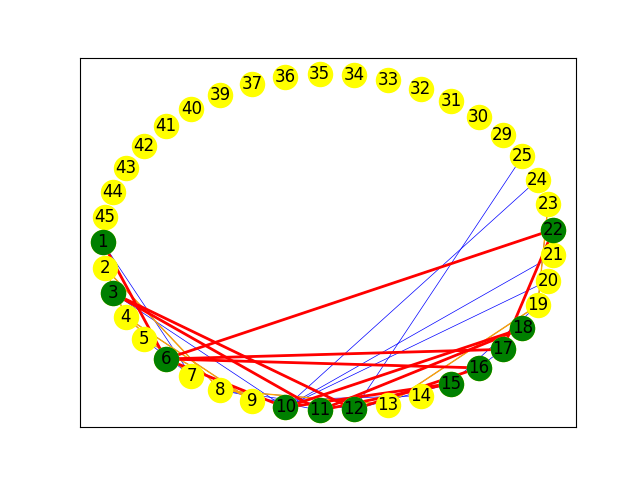
\includegraphics[width=0.7\linewidth]{images/sis2009/H_sis2009_cmp_acm68_m1_mcs_mix}
\caption{Sis2009 ACM68 MCS modelo 1}
\label{fig:modelo1}


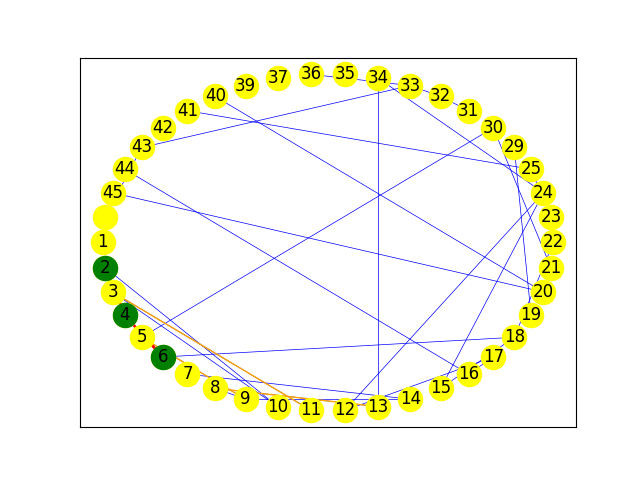
\includegraphics[width=0.7\linewidth]{images/sis2009/H_sis2009_cmp_acm68_m2_mcs_mix}
\caption{Sis2009 ACM68 MCS modelo 2}
\label{fig:modelo2}

\end{figure}

\begin{table}[H]
\centering
\caption{Tabulación de datos sobre comparaciones}
\begin{tabular}[t]{|l|l|l|l|l|l|}
\hline
Caso & Modelo & G(acm68)-n & G(acm68)-e & H(sis2009)-n & H(sis2009)-e\\
1&model1&30&39&41&34\\
\hline
1&model2&30&39&42&32\\
\hline
\end{tabular}
\label{tab:tabcomparaciones_P2}
\end{table}


\begin{table}[H]
\centering
\caption{Comparación G-ACM 68 y H-Sistemas 2009}
\begin{tabular}[t]{lccccc}
\hline
Caso & Modelo & MCSsubgrado & similaridad & nodos & enlaces \\
1 & $modelo_1 $ & 0.64285714 & $z=0.35714286$ & 11 & 13\\
1 & $modelo_2 $& 0.9285714286 & $z=0.07142857143$ & 3 & 2\\
\hline

\end{tabular}
\label{tab:tabcomparaciones_P2}
\end{table}

\begin{table}[H]
\centering
\caption{Tabla de resultados de proporcionalidad}
\begin{tabular}[t]{lccccccccc}
\hline
Caso & Modelo & nodosCom & enlacesCom & proporcionG &proporcionH \\
1 & $modelo_1$ & 20 & 21 & $t_1=0.6666666667$ & $t_2=0.487804878$ \\
1 & $modelo_2$ & 9 & 5 & $t_1=0.3 $ & $t_2=0.2142857143$ \\
\hline
\end{tabular}
\label{tab:tabresultados2_P2}
\end{table}

\begin{table}[H]
\centering
\caption{Tabla de Hipotesis vs Resultados }
\begin{tabular}[t]{lccccc}
\hline
Hipotesis & Caso & modelo & Similaridad & ProporcionG & ProporcionH\\
P2 & 1 & modelo1 & $z>0.2$ & $t_1>0.1$ & $t_2>0.1$ \\
P2 & 1 &modelo2 & $z<0.1$ & $t_1>0.1$ & $t_2<0.1$\\
\hline
\end{tabular}
\label{tab:hipotesis_P2}
\end{table}

\clearpage

\subsection{Caso 2 Hipotesis Secundaria 1}

A continuación se muestran las representaciones gráficas y los resultados del $Caso_2$ de la comparación entre un plan de estudio: Sistemas 2017 y la guía internacional ACM 68. Las comparaciones muestran en la figura \ref{fig:c2p2modelo1} la comparación asumiendo que los nodos respetan la red de relaciones de acm68 y en la figura \ref{fig:c2p2modelo2} se muestra el grafo considerando las relaciones 

\begin{figure}[H]
\centering
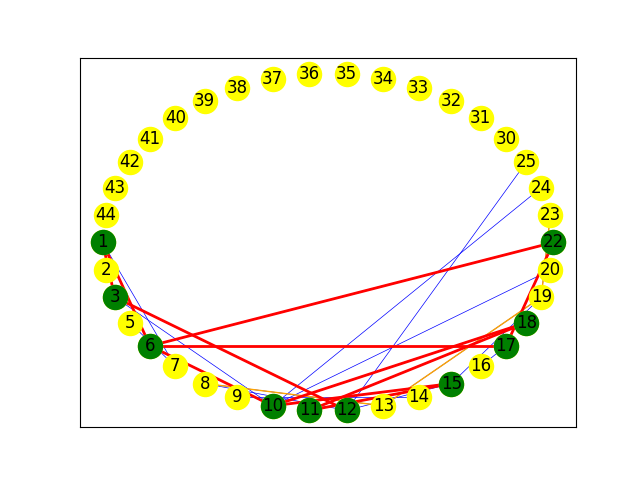
\includegraphics[width=0.7\linewidth]{images/sis2018/H_sis2018_acm68_m1_mcs_mix}
\caption{Sis2017 ACM68 MCS modelo 1}
\label{fig:c2p2modelo1}


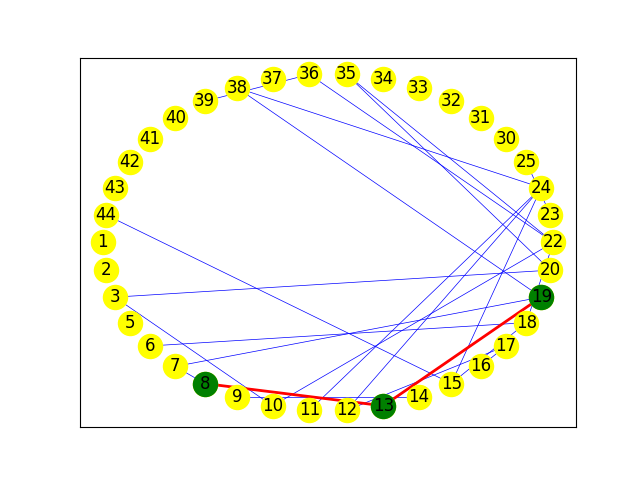
\includegraphics[width=0.7\linewidth]{images/sis2018/H_sis2018_acm68_m2_mcs_mix}
\caption{Sis2017 ACM68 MCS modelo 2}
\label{fig:c2p2modelo2}

\end{figure}


\begin{table}[H]
\centering
\caption{Tabulación de datos sobre comparaciones}
\begin{tabular}[t]{|l|l|l|l|l|l|}
\hline
Caso & Modelo & G(acm68)-n & G(acm68)-e & H(sis2009)-n & H(sis2009)-e\\
2&model1&30&39&38&25\\
\hline
2&model2&30&39&38&24\\
\hline
\end{tabular}
\label{tab:tabcomparaciones_C2_P2}
\end{table}


\begin{table}[H]
\centering
\caption{Comparación G-ACM 68 y H-Sistemas 2009}
\begin{tabular}[t]{lccccc}
\hline
Caso & Modelo & MCSsubgrado & similaridad & nodos & enlaces \\
2 & $modelo_1$ & 0.736842105263158 & $z=0.2631578947$ & 10 & 11\\
2 & $modelo_2$ & 0.9210526316 & $z=0.07894736842$ & 3 & 2\\
\hline
\end{tabular}
\label{tab:tabcomparaciones_C2_P2}
\end{table}

\begin{table}[H]
\centering
\caption{Tabla de resultados de proporcionalidad}
\begin{tabular}[t]{lccccccccc}
\hline
Caso & Modelo & nodosCom & enlacesCom & proporcionG &proporcionH \\
2 & $modelo_1$ & 14 & 14 & $t_1=0.4666666667$ & $t_2=0.3684210526$ \\
2 & $modelo_2$ & 3 & 2 & $t_1=0.1 $ & $t_2=0.07894736842$ \\
\hline
\end{tabular}
\label{tab:tabresultados2_C2_P2}
\end{table}

\begin{table}[H]
\centering
\caption{Tabla de Hipotesis vs Resultados }
\begin{tabular}[t]{lccccc}
\hline
Hipotesis & Caso & modelo & Similaridad & ProporcionG & ProporcionH\\
P2 & 2 & modelo1 & $z>0.2$ & $t_1>0.1$ & $t_2>0.1$\\
P2 & 2 & modelo1 & $z<0.2$ & $t_1>0.1$ & $t_2>0.1$\\
\hline
\end{tabular}
\label{tab:hipotesis_C2_P2}
\end{table}

\clearpage

\subsection{Caso 3 Hipotesis Secundaria 2}

A continuación se muestran las representaciones gráficas y los resultados del $Caso_3$ de la comparación entre un plan de estudio:  Ingeniería de Sistemas 2009 e Ingeniería de Sistemas 2017. Este caso se representa en la figura \ref{fig:c3p3modelo1} y en la figura \ref{fig:c3p3modelo2}. En la primera imagen se muestra una identificación del valor de similaridad teniendo como base al modelo de grafos del plan 2009. 

\begin{figure}[H]
\centering
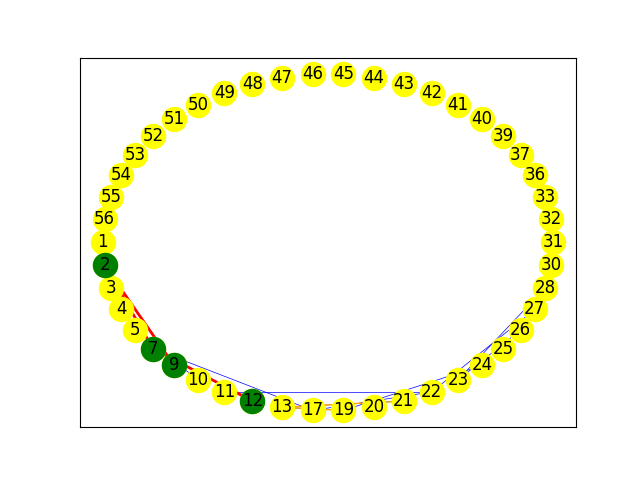
\includegraphics[width=0.7\linewidth]{images/sis2018/H_sis2018_cmp_sis2009_m1_mcs_mix}
\caption{Sis2009 Sis2017 MCS modelo 1}
\label{fig:c3p3modelo1}

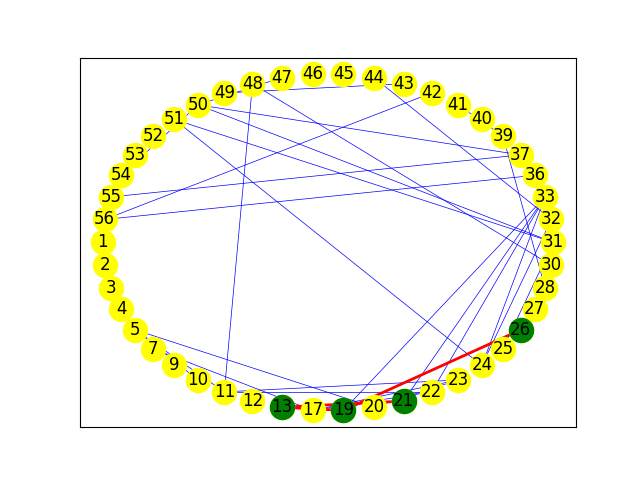
\includegraphics[width=0.7\linewidth]{images/sis2018/H_sis2018_cmp_sis2009_m2_mcs_mix}
\caption{Sis2009 Sis2017 MCS modelo 2}
\label{fig:c3p3modelo2}

\end{figure}


\begin{table}[H]
\centering
\caption{Tabulación de datos sobre comparaciones}
\begin{tabular}[t]{|l|l|l|l|l|l|}
3&model1&30&39&38&25\\
\hline
3&model2&30&39&38&24\\
\hline
\end{tabular}
\label{tab:tabcomparaciones_C_3_P3}
\end{table}


\begin{table}[H]
\centering
\caption{MCS}
\begin{tabular}[t]{lccccc}
\hline
Caso & Modelo & MCSsubgrado & similaridad & nodos & enlaces \\
3 & $modelo_1$ & 0.914893617 & $z=0.08510638298$ & 4 & 3 \\
3 & $modelo_2$ & 0.914893617 & $z=0.08510638298$ & 4 & 3 \\
\hline
\end{tabular}
\label{tab:tabcomparaciones_C_3_P3}
\end{table}

\begin{table}[H]
\centering
\caption{Tabla de resultados de proporcionalidad}
\begin{tabular}[t]{lccccccccc}
\hline
Caso & Modelo & nodosCom & enlacesCom & proporcionG &proporcionH \\
3 & $modelo_1$ & 7 & 5 & $t_1=0.1489361702$ & $t_2=0.152173913$\\
3 & $modelo_2$ & 4 & 3 & $t_1=0.08510638298$ & $t_2=0.08695652174$\\
\hline
\end{tabular}
\label{tab:tabresultados2_C_3_P3}
\end{table}

\begin{table}[H]
\centering
\caption{Tabla de Hipotesis vs Resultados }
\begin{tabular}[t]{lccccc}
\hline
Hipotesis & Caso & modelo & Similaridad & ProporcionG & ProporcionH\\
P3 & 3 & modelo1 &$z<0.2$&$t_1>0.1$&$t_2>0.1$\\
P3 & 3 & modelo1 &$z<0.2$&$t_1<0.1$&$t_2<0.1$\\
\hline
\end{tabular}
\label{tab:hipotesis_C_3_P3}
\end{table}


\clearpage

\subsection{Caso 4 Hipotesis Secundaria 2}

A continuación se muestran las representaciones gráficas y los resultados del $Caso_4$ de la comparación entre un plan de estudio: Ingeniería de sistemas 2017 y ACM 2013. En la figura \ref{fig:c4p2modelo1} se representa la comparación entre grafos priorizando los enlaces de ACM 2013 y en la figura \ref{fig:c4p2modelo2} cada grafo mantiene sus relaciones. 

\begin{figure}[H]
\centering
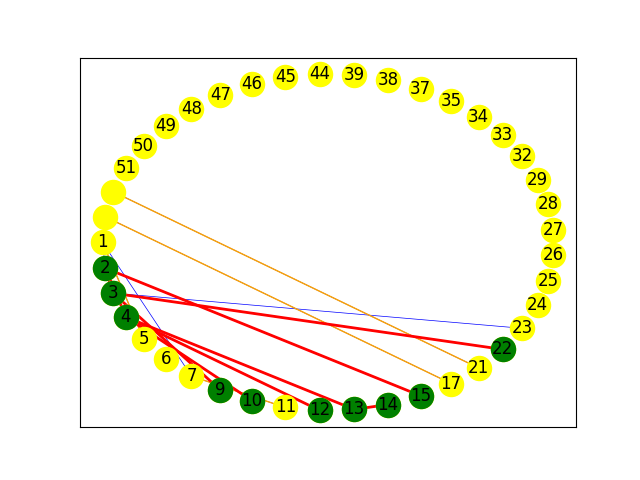
\includegraphics[width=0.7\linewidth]{images/sis2018/H_sis2018_cmp_acm2013_m1_mcs_mix}
\caption{Sis2017 y ACM 2013 MCS modelo 1}
\label{fig:c4p2modelo1}


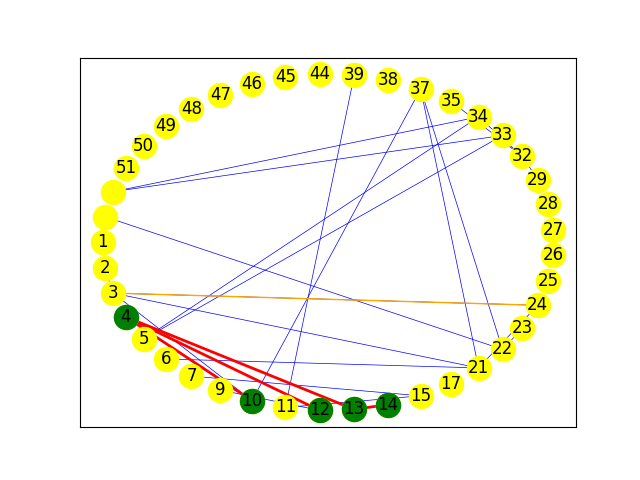
\includegraphics[width=0.7\linewidth]{images/sis2018/H_sis2018_cmp_acm2013_m2_mcs_mix}
\caption{Sis2017 y ACM 2013 MCS modelo 2}
\label{fig:c4p2modelo2}

\end{figure}


\begin{table}[H]
\centering
\caption{Tabulación de datos sobre comparaciones}
\begin{tabular}[t]{|l|l|l|l|l|l|}
\hline
4&model1&30&39&38&25\\
\hline
4&model2&30&39&38&24\\
\hline
\end{tabular}
\label{tab:tabcomparaciones_C4}
\end{table}


\begin{table}[H]
\centering
\caption{MCS}
\begin{tabular}[t]{lccccc}
\hline
Caso & Modelo & MCSsubgrado & similaridad & nodos & enlaces \\
4 & $modelo_1$ & 0.756097561 & $z=0.243902439$ & 10 & 9\\
4 & $modelo_2$ & 0.8780487805 & $z=0.1219512195$ & 5 & 4\\
\hline
\end{tabular}
\label{tab:tabcomparaciones_C4_P2}
\end{table}

\begin{table}[H]
\centering
\caption{Tabla de resultados de proporcionalidad}
\begin{tabular}[t]{lccccccccc}
\hline
Caso & Modelo & nodosCom & enlacesCom & proporcionG &proporcionH \\
4 & $Modelo_1$ & 18 & 13 & $t_1=0.75$ & $t_2=0.4390243902$\\
4 & $Modelo_2$ & 8 & 6 & $t_1=0.3333333333$ & $t_2=0.1951219512$\\
\hline
\end{tabular}
\label{tab:tabresultados2_C4_P2}
\end{table}

\begin{table}[H]
\centering
\caption{Tabla de Hipotesis vs Resultados }
\begin{tabular}[t]{lccccc}
\hline
Hipotesis & Caso & modelo & Similaridad & ProporcionG & ProporcionH\\
P2 & 4 & modelo1 &$z>0.02$&$t_1>0.1$&$t_2>0.1$\\
P2 & 4 & modelo1 &$z<0.02$&$t_1>0.1$&$t_2>0.1$\\
\hline
\end{tabular}
\label{tab:hipotesis_C4_P2}
\end{table}

\clearpage

\subsection{Caso 5 Hipotesis Secundaria 2}

A continuación se muestran las representaciones gráficas y los resultados del $Caso_5$ de la comparación entre un plan de estudio de ingeniería informática y una guía internacional ACM 2013. En la comparación del modelo 1, se representa con la figura \ref{fig:c5p2modelo1} con grafos y enlaces del modelo ACM y en la figura \ref{fig:c5p2modelo2} que representa cada grafo con sus respectivos enlaces. 

\begin{figure}[H]
\centering
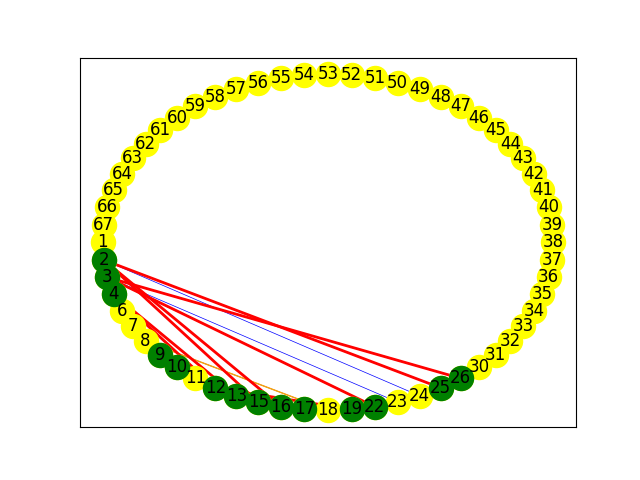
\includegraphics[width=0.7\linewidth]{images/pucp/H_pucp2020_cmp_acm2013_m1_mcs_mix.png}
\caption{IngInform2020 y ACM 2013 MCS modelo 1}
\label{fig:c5p2modelo1}


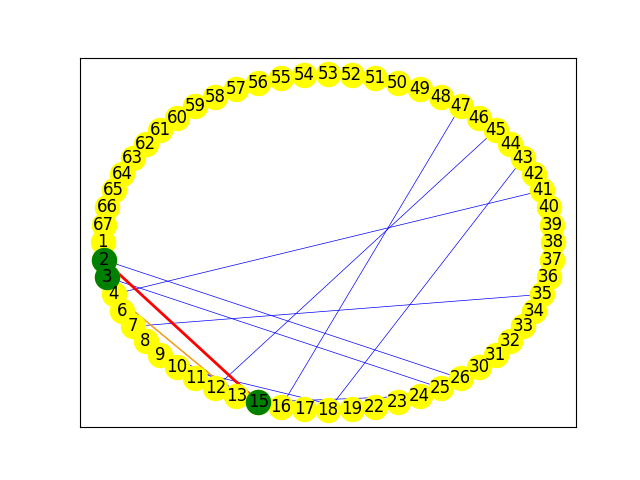
\includegraphics[width=0.7\linewidth]{images/pucp/H_pucp2020_cmp_acm2013_m2_mcs_mix.png}
\caption{IngInform2020 y ACM 2013 MCS modelo 2}
\label{fig:c5p2modelo2}

\end{figure}


\begin{table}[H]
\centering
\caption{Tabulación de datos sobre comparaciones}
\begin{tabular}[t]{|l|l|l|l|l|l|}
\hline
5&model1&26&20&60&20\\
\hline
5&model2&26&20&60&17\\
\hline
\end{tabular}
\label{tab:tabcomparaciones_C5}
\end{table}


\begin{table}[H]
\centering
\caption{MCS}
\begin{tabular}[t]{lccccc}
\hline
Caso & Modelo & MCSsubgrado & similaridad & nodos & enlaces \\
5 & $modelo_1$ & 0.766666666666666 & $z=0.2333333333$ & 18 & 16\\
5 & $modelo_2$ & 0.95 & $z=0.05$ & 5 & 3\\
\hline
\end{tabular}
\label{tab:tabcomparaciones_C5}
\end{table}

\begin{table}[H]
\centering
\caption{Tabla de resultados de proporcionalidad}
\begin{tabular}[t]{lccccccccc}
\hline
Caso & Modelo & nodosCom & enlacesCom & proporcionG &proporcionH \\
5 & $Modelo_1$ & 18 & 16 & $t_1=0.6923076923$ & $t_2=0.3$\\
5 & $Modelo_2$ & 5 & 3 & $t_1=0.1923076923$ & $t_2=0.08333333333$\\
\hline
\end{tabular}
\label{tab:tabresultados2_C5}
\end{table}

\begin{table}[H]
\centering
\caption{Tabla de Hipotesis vs Resultados }
\begin{tabular}[t]{lccccc}
\hline
Hipotesis & Caso & modelo & Similaridad & ProporcionG & ProporcionH\\
P2 & 5 & modelo1 &$z>0.02$&$t_1>0.1$&$t_2>0.1$\\
P2 & 5 & modelo1 &$z<0.02$&$t_1>0.1$&$t_2<0.1$\\
\hline
\end{tabular}
\label{tab:hipotesis_C5}
\end{table}


\clearpage


\subsection{Caso 6 Hipotesis Secundaria 1}

A continuación se muestran las representaciones gráficas y los resultados del $Caso_6$ de la comparación entre un plan de estudio de ingeniería de sistemas(UNI) y una guía internacional ACM 68. En la comparación del modelo 1, se representa con la figura \ref{fig:c6p1modelo1} con grafos y enlaces del modelo ACM y en la figura \ref{fig:c6p1modelo2} que representa cada grafo con sus respectivos enlaces. 

\begin{figure}[H]
\centering
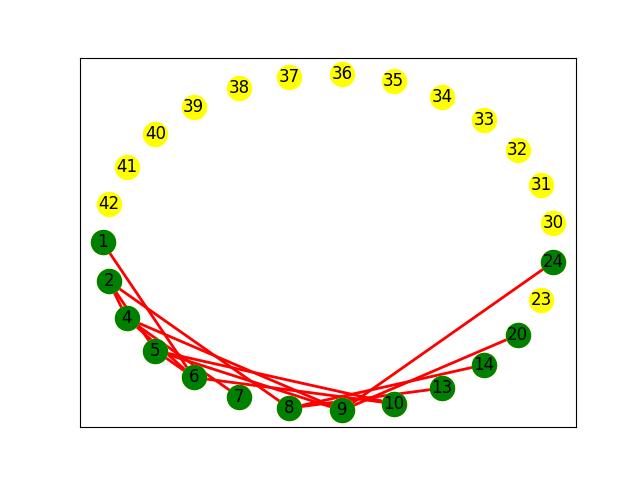
\includegraphics[width=0.7\linewidth]{images/sisuni2018/H_sisuni2018_cmp_acm68_m1_mcs_mix.png}
\caption{IngSistemas2018 y ACM 68 MCS modelo 1}
\label{fig:c6p1modelo1}


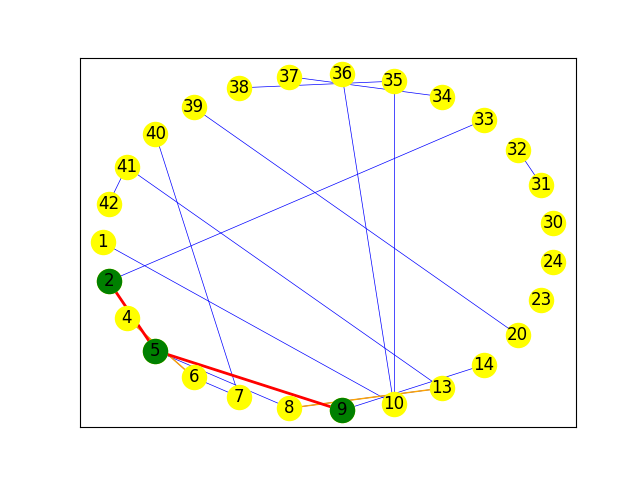
\includegraphics[width=0.7\linewidth]{images/sisuni2018/H_sisuni2018_cmp_acm68_m2_mcs_mix.png}
\caption{IngSistemas2018 y ACM 68 MCS modelo 2}
\label{fig:c6p1modelo2}

\end{figure}


\begin{table}[H]
\centering
\caption{Tabulación de datos sobre comparaciones}
\begin{tabular}[t]{|l|l|l|l|l|l|}
\hline
6&model1&30&39&27&15\\
\hline
6&model2&30&39&27&18\\
\hline
\end{tabular}
\label{tab:tabcomparaciones_C6}
\end{table}


\begin{table}[H]
\centering
\caption{MCS}
\begin{tabular}[t]{lccccc}
\hline
Caso & Modelo & MCSsubgrado & similaridad & nodos & enlaces \\
6 & $modelo_1$ & 0.566666666666667 & $z=0.4333333333$ & 13 & 15\\
6 & $modelo_2$ & 0.9 & $z=0.1$ & 3 & 2\\
\hline
\end{tabular}
\label{tab:tabcomparaciones_C6}
\end{table}

\begin{table}[H]
\centering
\caption{Tabla de resultados de proporcionalidad}
\begin{tabular}[t]{lccccccccc}
\hline
Caso & Modelo & nodosCom & enlacesCom & proporcionG &proporcionH \\
6 & $Modelo_1$ & 13 & 15 & $t_1=0.43$ & $t_2=0.3$\\
6 & $Modelo_2$ & 7 & 4 & $t_1=0.1$ & $t_2=0.08333333333$\\
\hline
\end{tabular}
\label{tab:tabresultados2_C5_P1}
\end{table}

\begin{table}[H]
\centering
\caption{Tabla de Hipotesis vs Resultados }
\begin{tabular}[t]{lccccc}
\hline
Hipotesis & Caso & modelo & Similaridad & ProporcionG & ProporcionH\\
P1 & 6 & modelo1 &$z>0.02$&$t_1>0.1$&$t_2>0.1$\\
P1 & 6 & modelo2 &$z<0.02$&$t_1<0.1$&$t_2<0.1$\\
\hline
\end{tabular}
\label{tab:hipotesis_C6}
\end{table}



\section{Resultados}

Como podemos observar no en todos los casos se logra obtener una similaridad mínima es decir cuando $z > 0.2 $ lo que invalida el caso de la hipótesis considerada en el estudio. El uso o no de las relaciones originales en la equivalencia de cursos. Es decir cuando usamos las relaciones originales de las curriculas internacionales se encuentra más casos de similaridad, pero también se encuentran casos que teniendo las relaciones del $Modelo_2$ se da un grado de similaridad. Esto es importante subrayar pues el modelamiento y la comparación nos puede dar pistas sobre que áreas y que cursos servirán como elementos para una incorporación o adaptación a perfiles de una curricula o guía internacional sin que eso afecte la estructura orgánica de la propuesta educativa.

En el caso del indicador $t > 0.1$ podemos observar el cumplimiento de los casos de proporcionalidad con mayor incidencia en el $Modelo_1$ eso nos da una pista que en algunos casos las relaciones de dependencia de las guías internacionales pueden acercar más la adopción de los referentes en contraste a que las instituciones usan sus propios esquemas de dependencia entre cursos, es decir no solo es necesario incorporar cursos y áreas de conocimiento sino también observar las dependencias entre estos cursos o contenidos. 


\clearpage

\section{Conclusiones}

\begin{enumerate}
	\item El modelamiento en grafos para la información de planes de estudio como de guias internacionales y habilitar la opción de comparación con indicadores numéricos es una herramienta novedosa para abordar el proceso de innovación curricular de las instituciones. 
	\item Más allá de las diferencias estructurales o históricas de las escuelas peruanas, utilizando herramientas como las propuestas en el presente estudio una institución puede observar el cambio en el tiempo y la adaptación a los distintos enfoques que va teniendo del diseño curricular. Además que puede observar si esa orientación refleja algún perfil o contenido central. El alcance de esta investigación no ha abordado la comparación en concreto de niveles de profundidad o tipos de orientación de los cursos, dado que eso implicaría un nivel más elaborado de comparaciones. Pero si se plantea el método y los mecanismos que pueden permitir ese nivel de evaluación de esos casos.
	\item El plantear comparaciones entre planes de estudio de la diversidad de oferta educativa así como encontrar similitudes con guías internacionales apoya la inclusión de los referentes internacionales así como puntos de partida para las instituciones.
	\item La inclusión de un modelo de referente internacional como el ACM68 y compararlo con al menos un plan de estudio antiguo de una universidad nos sirve para encontrar pistas de la influencia de la computación internacional en décadas pasadas y en parte también dar pistas que los planes de estudio pueden seguir la línea de profesiones de informática internacional así lleven nombres de profesiones de ingeniería.

\end{enumerate}

\newpage

\section{Trabajos futuros}

El mundo de la educación en informática es cambiante como la disciplina misma, mientras se le observa se va adaptando y cambiando en el tiempo. Sin embargo lo que menos cambia es la institucionalidad y eso se refleja tanto en los diseños orgánicos de las instituciones educativas como de los planes de oferta educativa, las personas y los elementos culturales. Innovar en estos sistemas sociales es un verdadero desafío que solo tiene sentido con el impulso de cada organización. Este estudio se presenta como una oportunidad para contribuir con herramientas de análisis cuantitativo en el estudio del desarrollo de los cambios y de la arquitectura interna de las relaciones de los contenidos y cursos de los programas educativos. Es un factor que no deberíamos ignorar como un elemento que nos permita contribuir en el desarrollo de los diseños curriculares y observar los movimientos y relaciones que puedan existir en los programas académicos.

Como trabajos futuros quedan poder hacer comparaciones a nivel de competencias de los planes de estudio y sus correspondientes guías internacionales o pares educativos. También poder hacer comparaciones a nivel de propiedades de los grafos, como por ejemplo el nivel de orientación teórico práctico de una grafo que corresponda a una unidad de conocimiento o curso. Poder realizar análisis de concentraciones o de agrupamientos de áreas también puede mejorar la toma de decisiones en la planificación educativa y vincular eso a otras necesidades económicas como industriales.

En cierta forma el modelamiento de los grafos y sus relaciones requiere juicio de análisis y por ende corre riesgo de introducir errores de interpretación, sin embargo esto puede reducirse conforme se puedan lograr consensos e interpretaciones por contenidos de los cursos. Es decir aplicando técnicas estadísticas y umbrales de aproximación en los contenidos de los cursos se podría lograr niveles de equivalencias entre nodos luego de las relaciones y poder ejecutar comparaciones más cercanas o automatizadas, introducir una capacidad de generalidad y escalamiento del proceso. 

Finalmente esta línea de investigación abre posibilidades para generar mejoras en la educación universitaria desde la comunidad académica de la informática en nuestras universidades.
%\bibliographystyle{utecbibstyle}
\bibliographystyle{apalike2}
\bibliography{biblio}

\appendix

\chapter{ANEXOS}

\section{Documento de codificación de datos}
\label{ane:anexo1}
Suspendisse eget faucibus sem, quis mattis lacus. Vivamus et leo molestie, suscipit tellus faucibus, finibus lacus. Phasellus non dolor cursus, pellentesque neque vel, condimentum tellus. Aliquam aliquam massa eget massa vestibulum gravida. Quisque quis arcu et orci porta sollicitudin eu vitae nunc. Aenean sed hendrerit eros. Sed auctor, tellus et suscipit ullamcorper, erat nisi luctus risus, id pulvinar leo massa sed libero. Interdum et malesuada fames ac ante ipsum primis in faucibus.citep{dataEstudio}


\section{Repositorio de imagenes y datos codificados}

Suspendisse eget faucibus sem, quis mattis lacus. Vivamus et leo molestie, suscipit tellus faucibus, finibus lacus. Phasellus non dolor cursus, pellentesque neque vel, condimentum tellus. Aliquam aliquam massa eget massa vestibulum gravida. Quisque quis arcu et orci porta sollicitudin eu vitae nunc. Aenean sed hendrerit eros. Sed auctor, tellus et suscipit ullamcorper, erat nisi luctus risus, id pulvinar leo massa sed libero. Interdum et malesuada fames ac ante ipsum primis in faucibus.





\end{document}